\chapter{Charm physics: quark mass and pseudoscalar decay constants}%\addcontentsline{toc}{chapter}{Light quark masses}
\label{ch_charm}

%%%%%%%%%%%%%%%%%%%%%%%%%%%%%%%%%%%%%%%%%%%%%%%%%%%%%%%%%%%
%%%%%%%%%%%%%%%%%%%%%%%%%%%%%%%%%%%%%%%%%%%%%%%%%%%%%%%%%%%
%%%%%%%%%%%%%%%%%%%%%%%%%%%%%%%%%%%%%%%%%%%%%%%%%%%%%%%%%%%
%%%%%%%%%%%%%%%%%%%%%%%%%%%%%%%%%%%%%%%%%%%%%%%%%%%%%%%%%%%

\section{Motivation}
\label{ch_qm:sec:introduction}

Blabla~\citep{charm}

Subset of CLS gauge ensembles, Table.

%%%%%%%%%%%%%%%%%%%%%%%%%%%%%%%%%%%%%%%%%%%%%%%%%%%%%%%%%%%
%%%%%%%%%%%%%%%%%%%%%%%%%%%%%%%%%%%%%%%%%%%%%%%%%%%%%%%%%%%
%%%%%%%%%%%%%%%%%%%%%%%%%%%%%%%%%%%%%%%%%%%%%%%%%%%%%%%%%%%
%%%%%%%%%%%%%%%%%%%%%%%%%%%%%%%%%%%%%%%%%%%%%%%%%%%%%%%%%%%

\section{Charm correlators}
\label{sec:charm_basics}

In this section we discuss the technical details behind the computation of physical observables in the charm region from our mixed action setup. We  introduce the GEVP setup used to extract meson masses and matrix elements throughout this work and explain our strategy to match the charm quark mass to its physical value.

\subsection{Computation of correlation functions}

In the charm region, the two-point functions defined in eq.~(\ref{ch_observables:eq:corrs}) are measured fixing the time position of the source at $y_0=T/2$, to maximise the distance from the boundaries: when dealing with heavy-light and heavy-heavy flavor contents in the correlators, we observe that the region in which the signal for the considered two-point function is accessible lies entirely within the lattice bulk, and that the boundary effects are strongly suppressed. Moreover, the numerical inversion of the quark propagator in the charm region is performed using distance preconditioning techniques~\cite{deDivitiis:2010ya,Collins:2017iud}, in order to reduce signal deterioration and enhance accuracy at large  Euclidean times.

In Sec.~\ref{ch_ma} we performed the matching of the sea and valence sectors of our mixed action for the light and strange flavors, in addition to tuning to maximal twist. Once the valence parameters were determined to ensure these conditions, an independent set of computations of heavy propagators was performed for the study of charm physics. Heavy propagators are computed at three different values of the twisted  mass $\mu_c^{(i)}$ around the physical charm region (save for one ensemble where only two masses have been used), so that observables are interpolated at the physical value of the charm quark mass. 

\subsection{Extraction of meson masses}
 
In our analysis meson masses are employed to fix the renormalised line of constant physics and match the quark masses to some target physical value.  Light and strange quark masses are matched between the sea and valence sectors using $\phi_2$ and $\phi_4$ in eqs.~(\ref{ch_ma:eq:phi2}-\ref{ch_ma:eq:phi4}), whereas for the partially quenched charm quark we use different combinations of mesons masses matched to their physical values, as explained in Sec.~\ref{subsec:matching_charm}.
 
The ground state meson masses involving heavy quarks are extracted from a generalised eigenvalue problem (GEVP) variational method defined as 
\begin{equation}\label{eq:gevp_sec3}
 	C(t) v_n(t,t_{\mathrm{ref}}) = \lambda_n(t,t_{\mathrm{ref}}) C(t_{\mathrm{ref}})v_n(t,t_{\mathrm{ref}}) \qquad n=0,\ldots,N-1 , \quad t>t_{\mathrm{ref}},
\end{equation}
where $C(t)$ is a matrix of Euclidean correlation functions of the form in eq.~(\ref{eq:f2p}), such that the indices $i,j$ in $C_{ij}(t)$ correspond to different choices of $\Gamma,\Gamma'$ and source/sink location, and $t=x_0-y_0$. This leads to the spectral expansion
\begin{gather}
\begin{split}
 	C_{ij}(t) &= \sum_{n=0}^{\infty} e^{-E_n t}\varphi_{ni} \varphi_{nj}^*, \quad i,j=0,\ldots, N-1 \,;\\
 \varphi_{ni} &\equiv \langle0|O_i|n\rangle.
\end{split}
\end{gather}
Here $N$ denotes the matrix dimension, and we have assumed non-degenerate energy levels. The GEVP  is solved in the regime  $t_{\mathrm{ref}} \geq t/2$, where a better control over excited state contributions is achieved \cite{Blossier:2009kd}.  The matrix $C(t)$ in our setup is built from pseudoscalar two-point functions $f_{\rm\scriptscriptstyle PP}$ shifted in time as
\begin{equation}
 	C_{\rm\scriptscriptstyle P}(t) = \bigg[\begin{matrix}
 		f_{\rm\scriptscriptstyle PP}(t)  &  f_{\rm\scriptscriptstyle PP}(t+\tau)
 		\\
 		f_{\rm\scriptscriptstyle PP}(t+\tau)  & f_{\rm\scriptscriptstyle PP}(t+2\tau)
 	\end{matrix}\bigg] \,,
\label{eq:gevp_matrix}
\end{equation}
where $\tau$ is the value of the time shift. Several values of the time shift have been tested, and we observe a mild dependence on small values of $\tau$ for the extraction of eigenvalues and eigenvectors. We refer to Appendix \ref{app:gevp} for a detailed discussion of our setup, together with sanity checks on the GEVP. In what follows we set $\tau=3a$.
  
The ground state meson mass is extracted from the eigenvalues of the GEVP using eq.~(\ref{eq:eff_en_gevp}). 
In order to assess the systematic effects and correctly identify the plateau region, following the same procedure we applied for lattice observables involving only light and strange flavors (see Sec.~\ref{ch_observables}) we perform several uncorrelated $\chi^2$ fits to a constant, by varying the time ranges of the fitting interval, and we eventually extract our ground state masses by means of the model averaging procedure described in Appendix~\ref{app:TIC}. An example of a GEVP plateau for the heavy-light pseudoscalar mass together with a summary of the model average procedure for an ensemble used in the analysis is shown in Figure \ref{fig:meff_plateau}. 
  
\begin{figure}
  	\centering
  	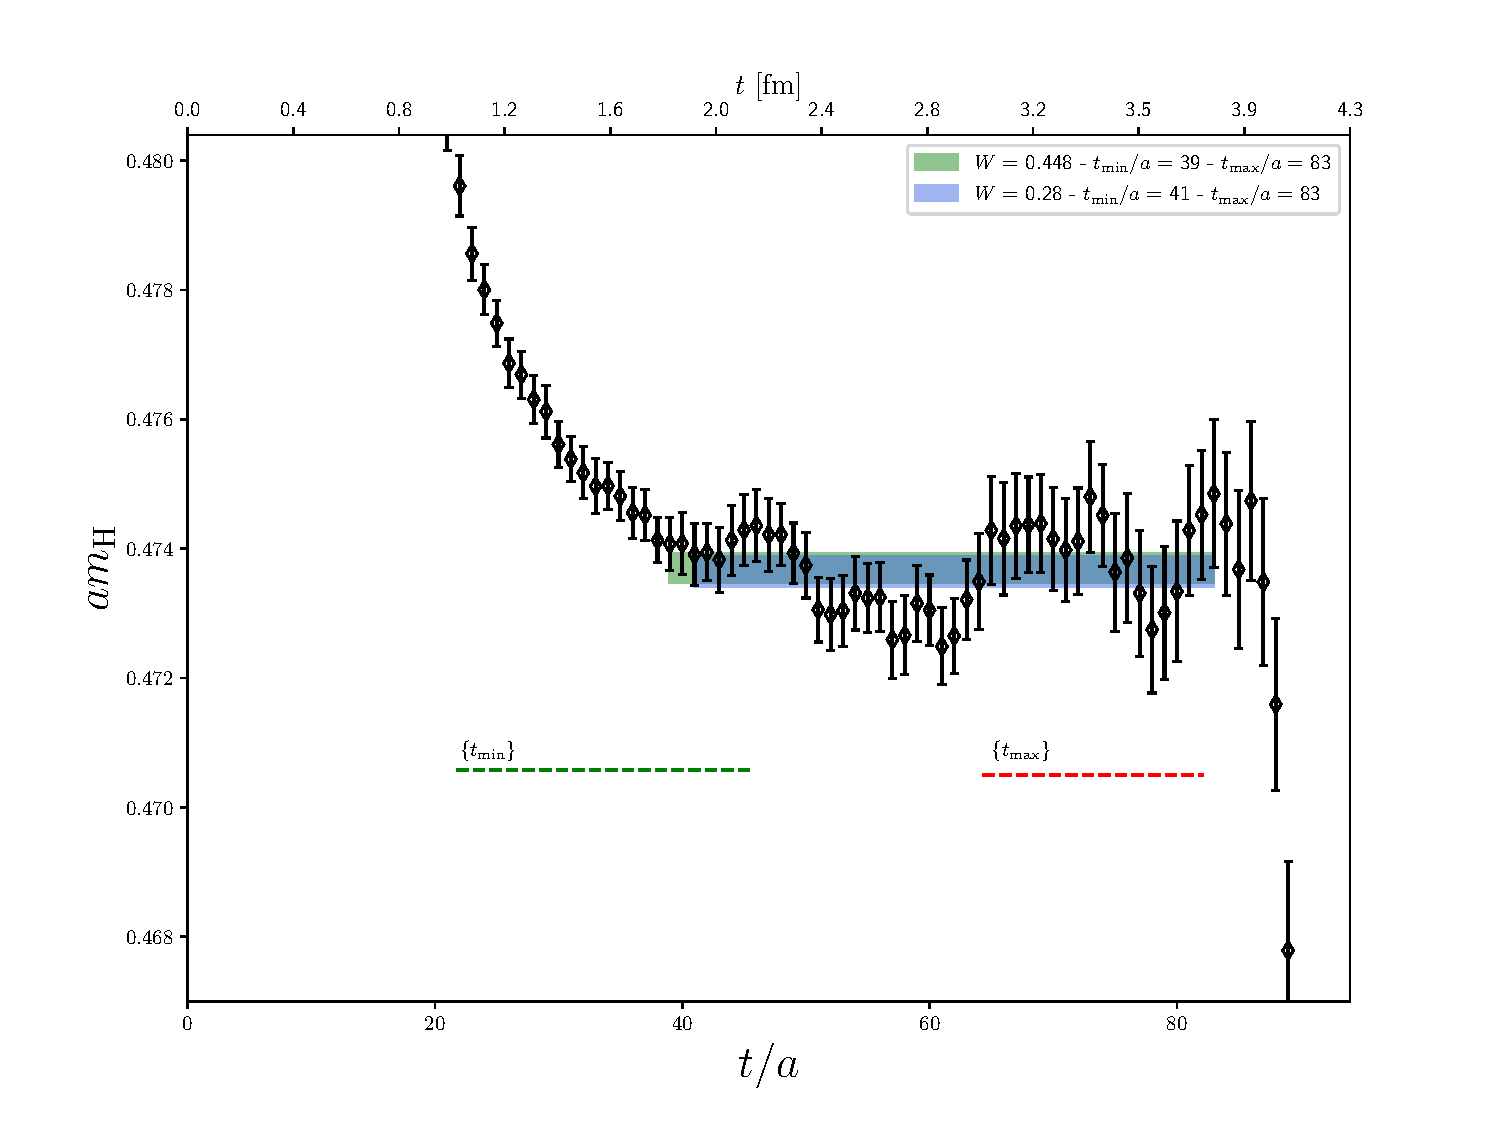
\includegraphics[scale=0.5]{./cap6/figs/matching/m8_plateau.pdf}
  	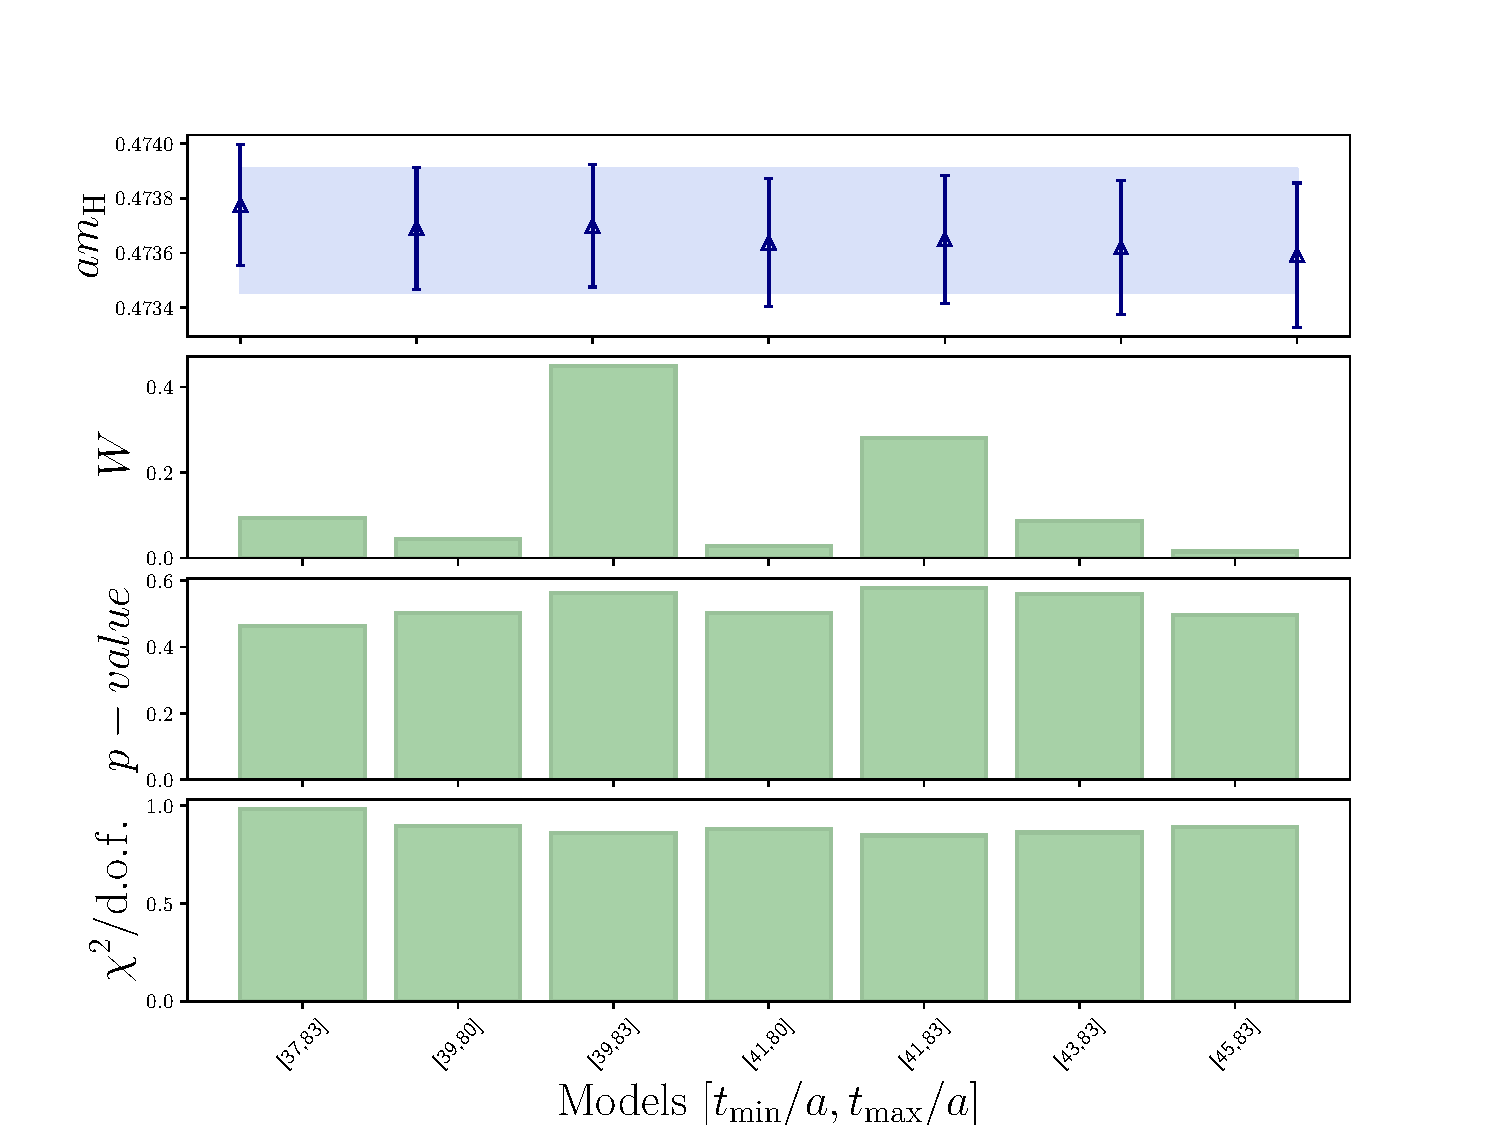
\includegraphics[scale=0.5]{./cap6/figs/matching/mps_BMA_8.pdf}
  	\caption{Illustration of the extraction of the ground-state mass after applying a GEVP analysis, illustrated for the ensemble J303. \textit{Top}: Heavy-light pseudoscalar meson mass plateau showing the  two fit intervals with higher weights $W$ contributing to the model average. We also indicate the range of variations allowed for the interval in Euclidean time where the plateau is taken. \textit{Bottom}: Summary of determinations of $am_{\mathrm H}$ when considering variations over the fit intervals $[t_{\rm min}/a, t_{\rm max}/a]$ together with  the corresponding normalised weights $W$ based on Takeuchi's Information Criterion (TIC), p-values and $\chi^2/{\rm d.o.f.}$. In the upper panel, the shaded blue band  corresponds to the model average result.} 
\label{fig:meff_plateau} 
\end{figure}
  


\subsection{Matching of the charm quark mass}
\label{subsec:matching_charm}
In Sec.~\ref{ch_ma} we recalled the matching of the light sector, which ensures that physical observables involving only light and strange quarks computed in the valence and sea sectors coincide up to cutoff effects, so that unitarity is recovered in the continuum limit.
%
A similar procedure is needed for the charm quark, designed to ensure that its physical value is obtained upon taking the continuum limit and performing chiral fits.
%
Since the charm is partially quenched this matching procedure involves observables with only valence charm quark propagators.
%

%
In order to establish a connection with the physical point, we require that some charm-like observable $O_c$ matches its physical value.
%
In this paper we studied three different charm scale settings based on three choices of $O_c$, all in terms of meson masses; we will denote the latter as $m_H^{(i)},~i=1,2,3$, and often express them in units of $\sqrt{8t_0}$ as $\phi_H^{(i)} = \sqrt{8t_0}m_H^{(i)}$.
%

The first possibility, corresponding to $\phi_H^{(1)}$, consists in using the flavour average meson mass combination
\begin{equation}
        m_H^{(1)} = m_{\overline{H}} \equiv \frac{2}{3} m_H + \frac{1}{3}m_{H_s},
        \label{eq:fl_av_matching}
\end{equation}
built from heavy-light $H$ and heavy-strange $H_s$ pseudoscalar meson masses with heavy-quark masses in neighbourhood of the charm.
%
Since we require the considered CLS ensembles to hold a constant value of the flavour average combination of pion and kaon masses -- denoted as $\phi_4$ in Eq.~(\ref{eq:phi2_and_phi4}) -- we also expect the flavour average combination  $\phi_H^{(1)}$ to remain fairly constant along the chiral trajectory. The physical value of $m_H^{(1), \mathrm{phys}}$ is obtained by setting $m_{H_{(s)}}$ to the following prescription for the isoQCD values of $D_{(s)}$ meson masses,
%
\begin{equation}
    m_D^{\mathrm{isoQCD}} = 1867.1 \pm 2.6  \ \mathrm{MeV}, \qquad m_{D_s}^{\mathrm{isoQCD}} = 1967.1 \pm 1.3 \ \mathrm{MeV}.
\label{eq:DsisoQCDinputs}
\end{equation}
%
  The uncertainties in these isoQCD values are chosen to cover the deviation with respect to the experimental values~\cite{ParticleDataGroup:2022pth} of the $D^{\pm}$ and $D_s^{\pm}$ meson masses, $m_{D^\pm}^{\mathrm{exp}} = 1869.66(5) \ \mathrm{MeV}$ and $m_{D_s^\pm}^{\mathrm{exp}} = 1968.35(7) \ \mathrm{MeV}$, respectively. We observe that the larger uncertainty in the isoQCD inputs of the $D$ and $D_s$ meson masses in Eq.~(\ref{eq:DsisoQCDinputs}) --- as compared to the corresponding experimental values --- does not induce a significant increase in the uncertainties of our target results. The input values in Eq.~(\ref{eq:DsisoQCDinputs}) lead to the following flavour averaged meson mass,
%
\begin{equation}
         m_H^{(1), \mathrm{phys}} = m_{\overline{D}} = 1900.4(1.8) \ \mathrm{MeV}\,.
\end{equation}
% 

Our second strategy, corresponding to $\phi_H^{(2)}$, is to
consider the mass-degenerate pseudoscalar meson mass $m_{\eta_h}^{\mathrm{conn}}$ extracted from
the quark-connected two-point correlation function made of heavy quark
propagators with a mass in the neighbourhood of the charm mass,
%
\begin{equation}
  m_H^{(2)} = m_{\eta_h}^{\mathrm{conn}}\,.
                  \label{eq:etac_matching}
\end{equation}
%
The physical value for this mass, $m_H^{(2), \mathrm{phys}}$,  is set from the experimental
value of the $\eta_c$ meson mass~\cite{ParticleDataGroup:2022pth},
$m_{\eta_c}^{\mathrm{exp}} = 2983.9(4)\,\MeV$, from which a
correction of about 6\,\MeV, with 100\% error, is subtracted to account
for the absence of quark-disconnected diagrams and QED effects~\cite{deForcrand:2004ia, Donald:2012ga,Colquhoun:2015oha,Hatton:2020qhk,Colquhoun:2023zbc}. Specifically, we employ, 
%
\begin{equation}
  m_H^{(2), \mathrm{phys}} = m_{\eta_c}^{\mathrm{conn}} = 2978(6) \ \mathrm{MeV}\,.
\end{equation}
%
One potential advantage of this choice of matching observable is that
the overall precision of the $\eta_c^{\mathrm{conn}}$ meson mass is substantially better than the one
for heavy-light meson masses, as it does not suffer from the increase in noise-to-signal
ratio with Euclidean time; this is illustrated in Figure \ref{fig:corr_comparison},
where we show the $D$, $D_s$ and $\eta_c^{\mathrm{conn}}$ pseudoscalar correlators for a one specific ensemble.
%
Finally, as a third matching quantity we also tested the spin-flavour averaged mass combination
 \begin{equation}
 	m_H^{(3)} = m_{\overline{H}^*} = \frac{1}{12} \left(
 	2m_H + m_{H_s} + 6 m_{H^*} + 3 m_{H_s^*}
 	\right),
 	\label{eq:spin_flavour_av}
 \end{equation}
which involves a combination of heavy-light pseudoscalar  $m_{H_{(s)}}$ and vector  $m_{H_{(s)}^*}$ meson masses in the charm region, and
is motivated by heavy-quark symmetry. However, we observe that chiral-continuum fits coming from the spin flavour-averaged matching condition
lead to worse $\chi^2$ values, and as a result their weights are highly suppressed by  our model average prescription. We interpret this finding as a reflection of relatively poor control of heavy-light vector states, whose masses are extracted with significantly larger errors than those of heavy-light pseudoscalar states (cf. Fig.~\ref{fig:mps_vs_mvec_gevp}). In the rest of the discussion we will therefore focus on the results coming from the other two matching conditions.
%

%
Any of these matching conditions can in principle be imposed ensemble by ensemble,
even away from the physical point.
%
However, by doing so we would as a result build in the charm quark mass a dependence on the value of
the reference scale $t_0^{\mathrm{phys}}$, as well as $O(a^2)$ effects coming from the
specific choice of $O_c$.
%
To avoid this, we have opted instead for setting the physical charm quark mass
jointly with the chiral-continuum
extrapolation, in a similar way as the one we employ to hit the physical point in the
light and strange sector.
%
What this means in practice is that the charm quark mass dependence of any given observable
$\cO$ is parameterised as $\mathcal{O}(a, \phi_2, \phi_H^{(i)})$, and we perform a global
fit to obtain its physical value $\mathcal{O}(0, \phi_2^{\mathrm{phys}}, \phi_H^{(i),\mathrm{phys}})$.
%
This will be the procedure applied below in the determination of the physical value of
the charm quark mass and of the decay constants $f_D$ and $f_{D_s}$.
%

%
Note that, as a consequence of our matching procedure and of working on a line of constant
physics where $\phi_4$ is kept constant, it is non-trivial that by adopting any of our 
matching procedures the mass of any particular meson reaches its physical value in the
chiral-continuum limit;
checking that it does is therefore a test of the robustness of our procedure.
%
As an illustration, we show in Fig.~\ref{fig:ds_matching} how the physical values
of the $D$ and $D_s$ meson masses arise when the charm scale is matched through either
$m_{\overline D}$ or $m_{\eta_c}^{\mathrm{conn}}$.
%
In either case we show results for the specific model of the lattice spacing, charm mass and pion mass
dependence of the form
\begin{equation}
\sqrt{8t_0}\, m_{D_{(s)}}(a, \phi_2, \phi_H^{(i)}) = p_0 + p_1\phi_2 +  p_2 \phi_H^{(i)} + c_1\frac{a^2}{8t_0},
\end{equation}
where $i=1,2$ according to the notation introduced above and where $c_1$ and $p_j$, $j=1,2,3$, stand for the fit parameters.
%
Note that the agreement is excellent, in spite of the different implications of the
two setups for the specific case of $m_{D_{(s)}}$; for instance, when $m_{\overline D}$ is used
for the matching cutoff effects are very small by construction, while the use of
$m_{\eta_c}^{\mathrm{conn}}$ leads to sizeable cutoff effects which are however
very well described by an $\mathcal{O}(a^2)$ term.


   
   \begin{figure}[!t]
   	\centering
   	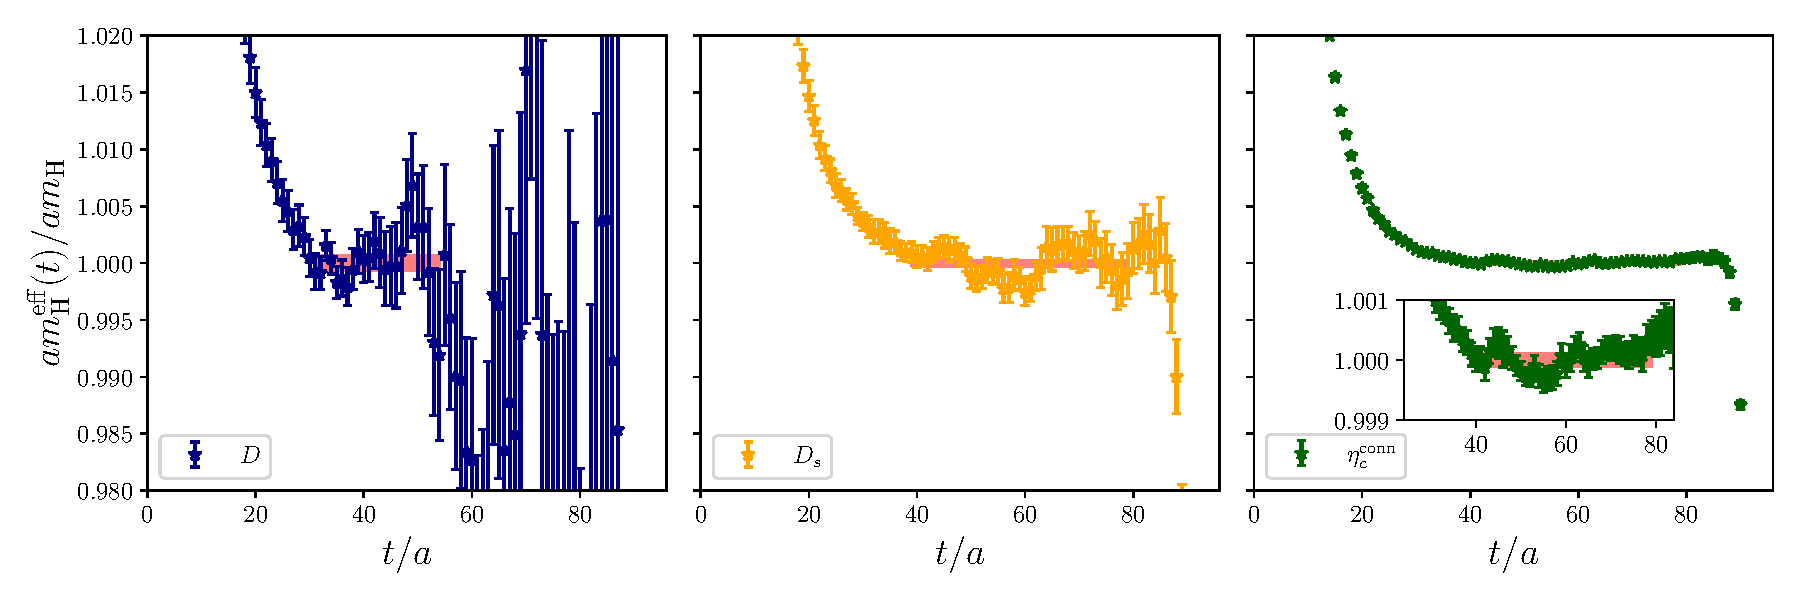
\includegraphics[scale=0.52]{./cap6/figs/matching/meff_comparison.pdf}
   	\caption{Illustration of the effective meson masses involved in the matching procedure to the physical charm scale for the ensemble J303. We show three cases where the effective mass of the pseudoscalar meson $H$ is that of the $D$ (\textit{left}), $D_s$ (\textit{center}) and $\eta_c^{\mathrm{conn}}$  (\textit{right}), normalised by the central value of the corresponding plateau averaged mass.  The horizontal red bands show the results of the highest weight fit contributing to the model average procedure and the corresponding plateau interval. We observe the expected increase of the statistical uncertainties at large time separations when increasing the mass-difference among the quarks propagators of the pseudoscalar two-point correlators. 
}
   	\label{fig:corr_comparison}
   \end{figure}
   
 \begin{figure}[!t]
 	\centering
 	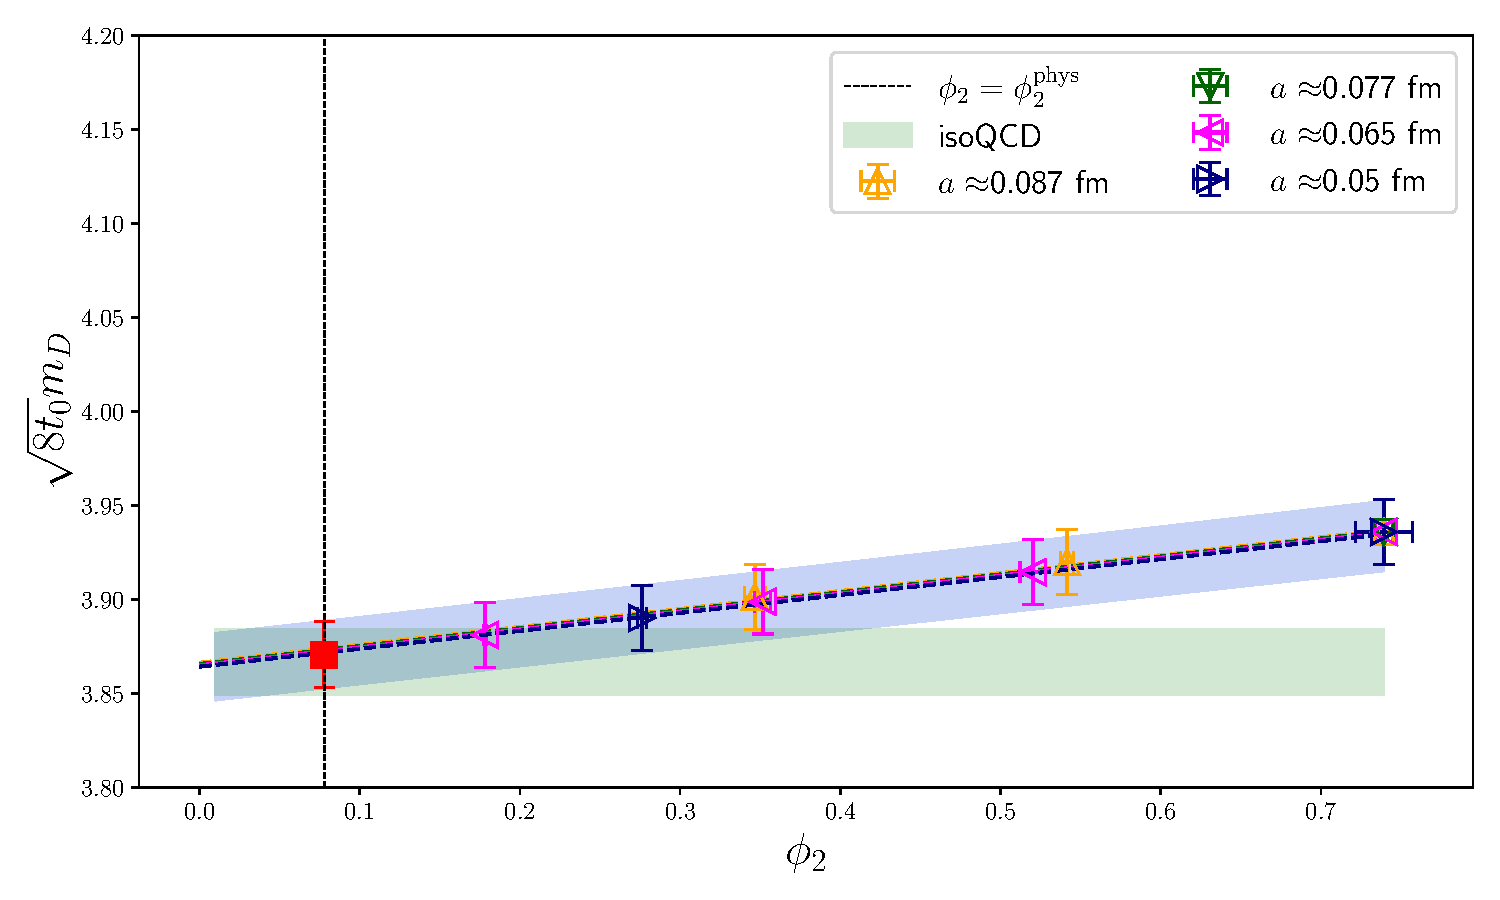
\includegraphics[scale=0.3]{./cap6/figs/matching/fit_phi2_mD_fl_ave.pdf}
 	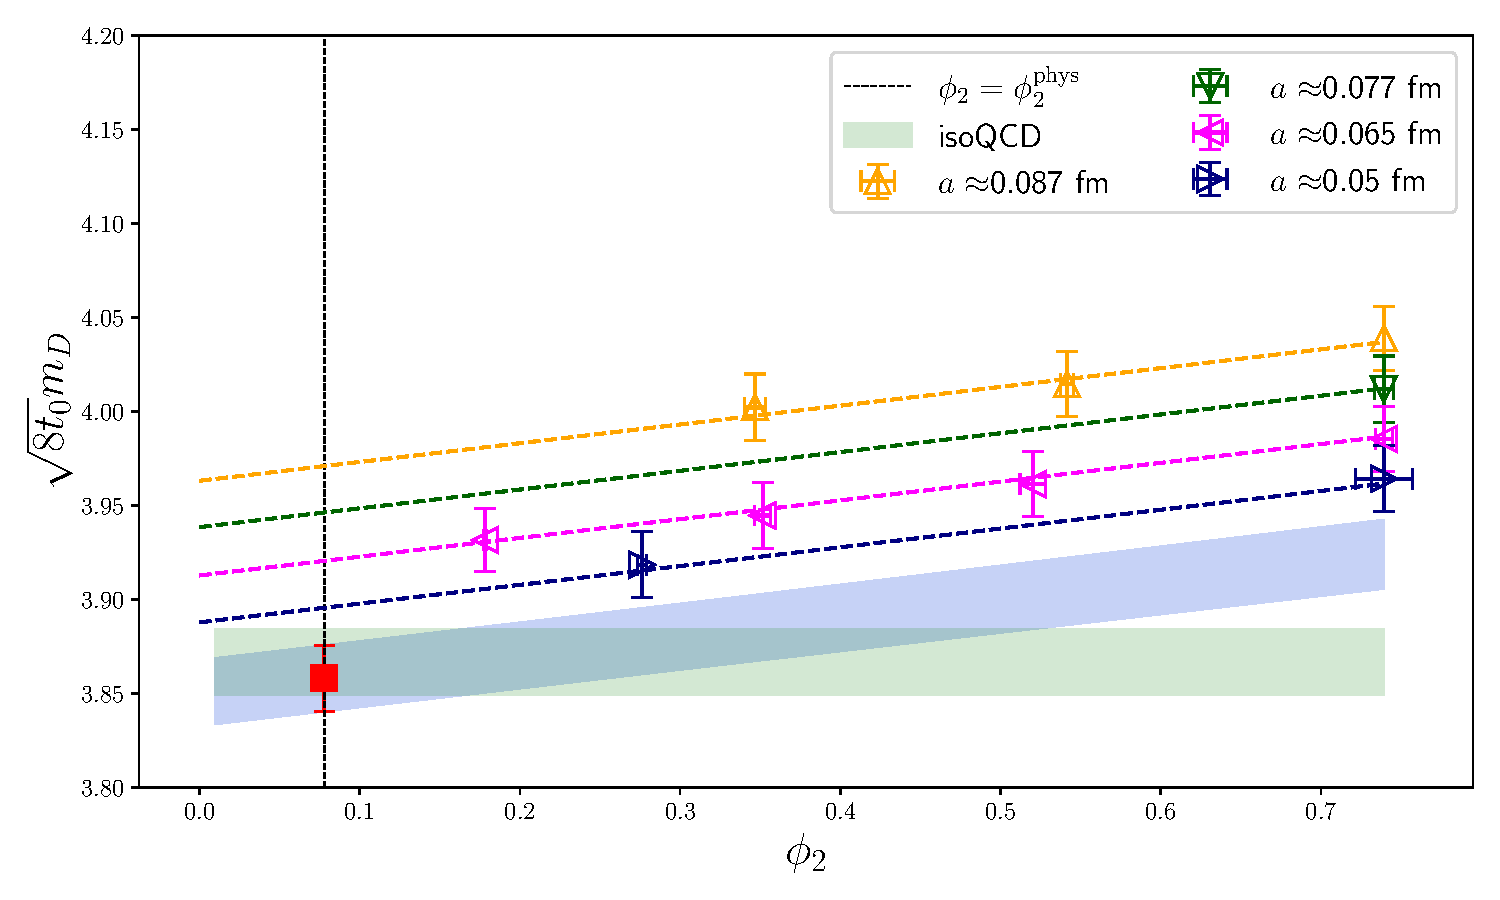
\includegraphics[scale=0.3]{./cap6/figs/matching/fit_phi2_mD_etac.pdf}
 	\\
 	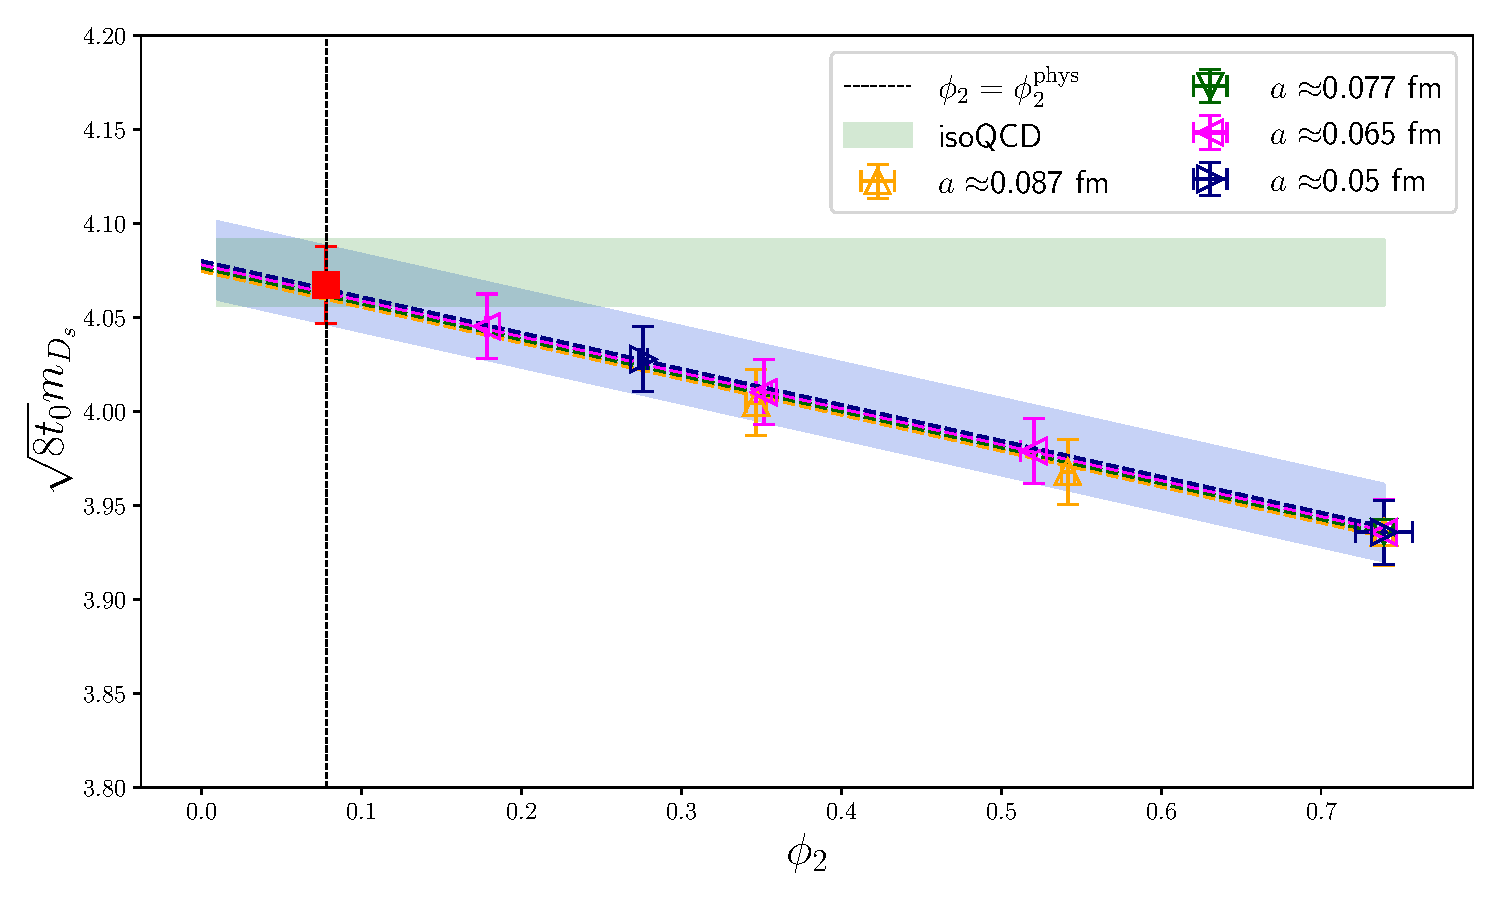
\includegraphics[scale=0.3]{./cap6/figs/matching/fit_phi2_mDs_fl_ave.pdf}
 	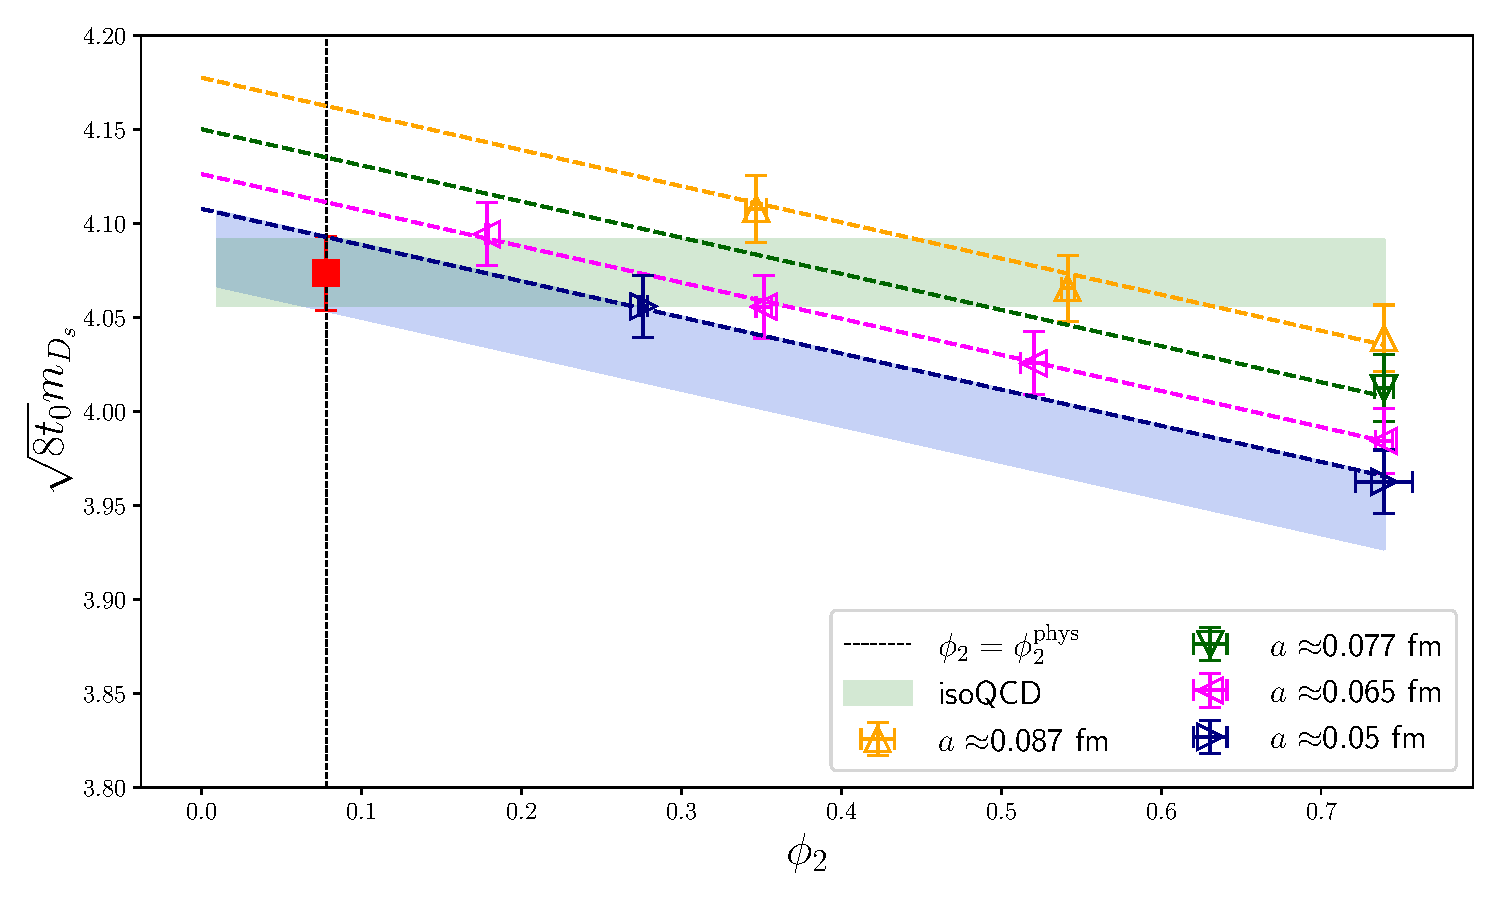
\includegraphics[scale=0.3]{./cap6/figs/matching/fit_phi2_mDs_etac.pdf}
 	\caption{Consistency checks of our charm matching strategy. We show the chiral extrapolation to the physical point of
	the ${D_{(s)}}$ meson mass in units of $\sqrt{8t_0}$ using all the ensembles listed in Table \ref{tab:CLS}.
	The left panels use the flavour-averaged mass combination, $m_H^{(1)}= m_{\overline{H}}$, while those on the right
	use the mass-degenerate pseudoscalar meson mass, $m_H^{(2)}=m_{\eta_h}^{\mathrm{conn}}$. The empty symbols correspond to the $D_{(s)}$ meson masses determined on a given ensemble,
	while the red square symbols show the extrapolated values at the physical point. Dashed lines
	show the fit forms projected to each individual lattice spacing, and the blue shaded bands
	are a projection to the continuum limit on the chiral plane. Data points are projected to the physical point $\phi_H^{(i),\mathrm{phys}}$. Finally, the green horizontal band shows
	the isoQCD input values for the corresponding masses in Eq.~(\ref{eq:DsisoQCDinputs}), in units of $\sqrt{8t_0}$.
        }
 	\label{fig:ds_matching} 
 \end{figure}

%%%%%%%%%%%%%%%%%%%%%%%%%%%%%%%%%%%%%%%%%%%%%%%%%%%%%%%%%%%
%%%%%%%%%%%%%%%%%%%%%%%%%%%%%%%%%%%%%%%%%%%%%%%%%%%%%%%%%%%
%%%%%%%%%%%%%%%%%%%%%%%%%%%%%%%%%%%%%%%%%%%%%%%%%%%%%%%%%%%
%%%%%%%%%%%%%%%%%%%%%%%%%%%%%%%%%%%%%%%%%%%%%%%%%%%%%%%%%%%

\section{Determination of the charm quark mass}
\label{sec:mc}

\subsection{Renormalised charm quark masses}

%
In Sec.~\ref{sec:mixed_action_setup} we have summed up the argument why renormalised quark
masses can be easily retrieved from bare Lagrangian twisted masses.
%
In our mixed-action setup, as discussed in detail in~\cite{MA1}, the resulting $O(a)$-improved expression for the renormalised  charm mass $\mbar_c(\mu)$ reads
\begin{equation}
	\mbar_c(\mu) = 
	 \ZP^{-1}(g_0^2, a\mu) [1 + a\overline{b}_\mu(g_0^2) \rm{tr}\{\mathbf{m}^{(s)}\}]\,\mu_c\,,
	\label{eq:renormalised_charm_mass}
\end{equation}
where $\ZP(g_0^2, a\mu)$ is a suitably defined renormalisation constant for the non-singlet
pseudoscalar density at renormalisation scale $\mu$.
%
As we have already discussed, the improvement term $\propto\rm{tr}\{\mathbf{m}^{(s)}\}$
can be neglected in practice, so $O(a)$-improved renormalised quark masses can be obtained
by just applying the renormalisation constants to the exactly known Lagrangian masses.
%


%
In this work we will use the non-perturbative values of $\ZP$ computed in~\cite{Campos:2018ahf}
in the Schr\"odinger Functional scheme, at a fixed renormalisation scale
$\mu_{\rm\scriptscriptstyle had} = 233(8)~\MeV$ and for the range of values of $g_0^2$ covered
by CLS.
%
It will be used to obtain renormalised quark masses for each of our ensembles, that can then
be used to determine the value of the charm quark mass in the continuum and at physical kinematics.
%
Contact with other renormalisation schemes can then be made by computing the renormalisation
group invariant (RGI) quark mass $M_c^{\mathrm{RGI}}$, using the continuum (flavour-independent)
ratio also computed in~\cite{Campos:2018ahf}
\begin{equation}
	\frac{M}{\overline{m}(\mu_{\mathrm{had}})} = 0.9148(88)\,.
	\label{eq:rgi_running_factor}
\end{equation}
%
Values of renormalised masses in, say, the $\MSbar$ scheme can then be obtained by
using the perturbative value of $\frac{\overline{m}(\mu)}{M}$ at any convenient scale $\mu$.
%

%%%%

\subsection{Charm quark mass chiral-continuum fits}
\label{subsec:mc_chiral_continuum}

Having determined the  renormalised charm quark masses in the Schr\"odinger Functional scheme at the hadronic renormalisation scale $\mu_{\mathrm{had}}$
\begin{equation}
\mbar_c(\mu_{\rm\scriptscriptstyle had}) \equiv \mu_c^{\rm\scriptscriptstyle R}\,,
\end{equation}
for all the ensembles listed in Table \ref{tab:CLS}, we now describe our 
strategy to obtain results in the continuum limit and at the physical point,
following the approach outlined in Sec.~\ref{sec:charm_basics}. The matching procedure of the light
and strange sectors is already devised so that the physical value of the kaon mass is recovered
at $\phi_2 = \phi_2^{\mathrm{phys}}$, where the physical value of $\phi_2$ is computed
with the isospin-symmetric values of the pion mass quoted 
in~\cite{FlavourLatticeAveragingGroupFLAG:2021npn}, and the physical scale $t_0^{\mathrm{phys}}$
is the one determined in~\cite{MA1}. The charm scale is matched through the two different
prescriptions described in Sec.~\ref{sec:charm_basics}. All quantities entering the fit
are made dimensionless through the appropriate power of the factor $\sqrt{8t_0}$,
and physical units for the final result are restored by using our value for $t_0^{\mathrm{phys}}$.

We parameterise the continuum dependence of the renormalised charm quark mass on $\phi_2$
and any of the $\phi_H^{(i)}$ with the functional form
\begin{equation}
	\sqrt{8t_0}\, \mu_c^{\rm\scriptscriptstyle R}(a=0, \phi_2, \phi_H) = p_0 + p_1\phi_2 + p_2\phi_H\,.
	\label{eq:mc_continuum_parameterization}
\end{equation}
Based on the heavy quark effective theory expansion~\cite{Georgi:1990um} at lowest order,
we expect a linear dependence of the charmed meson masses as a function of the the charm quark 
mass, hence the latter term in the ansatz. This assumption is supported by our data that show indeed a 
linear behaviour in the charmed meson masses, as illustrated in Figure \ref{fig:mc_mh_dependence}. Note that this form is used only to describe the dependence
within a short interval in mass values, and interpolate the charm scale from points close by. When considering the pion dependence of the charm quark mass, we assume that the  leading order contributions exhibit a linear behaviour in $\phi_2$. With the current set of ensembles employed in this work we do not observe any deviations from the leading order term in the pion mass dependence.

 \begin{figure}[!htb]
 	\centering
 	%\hspace{-15mm}
 	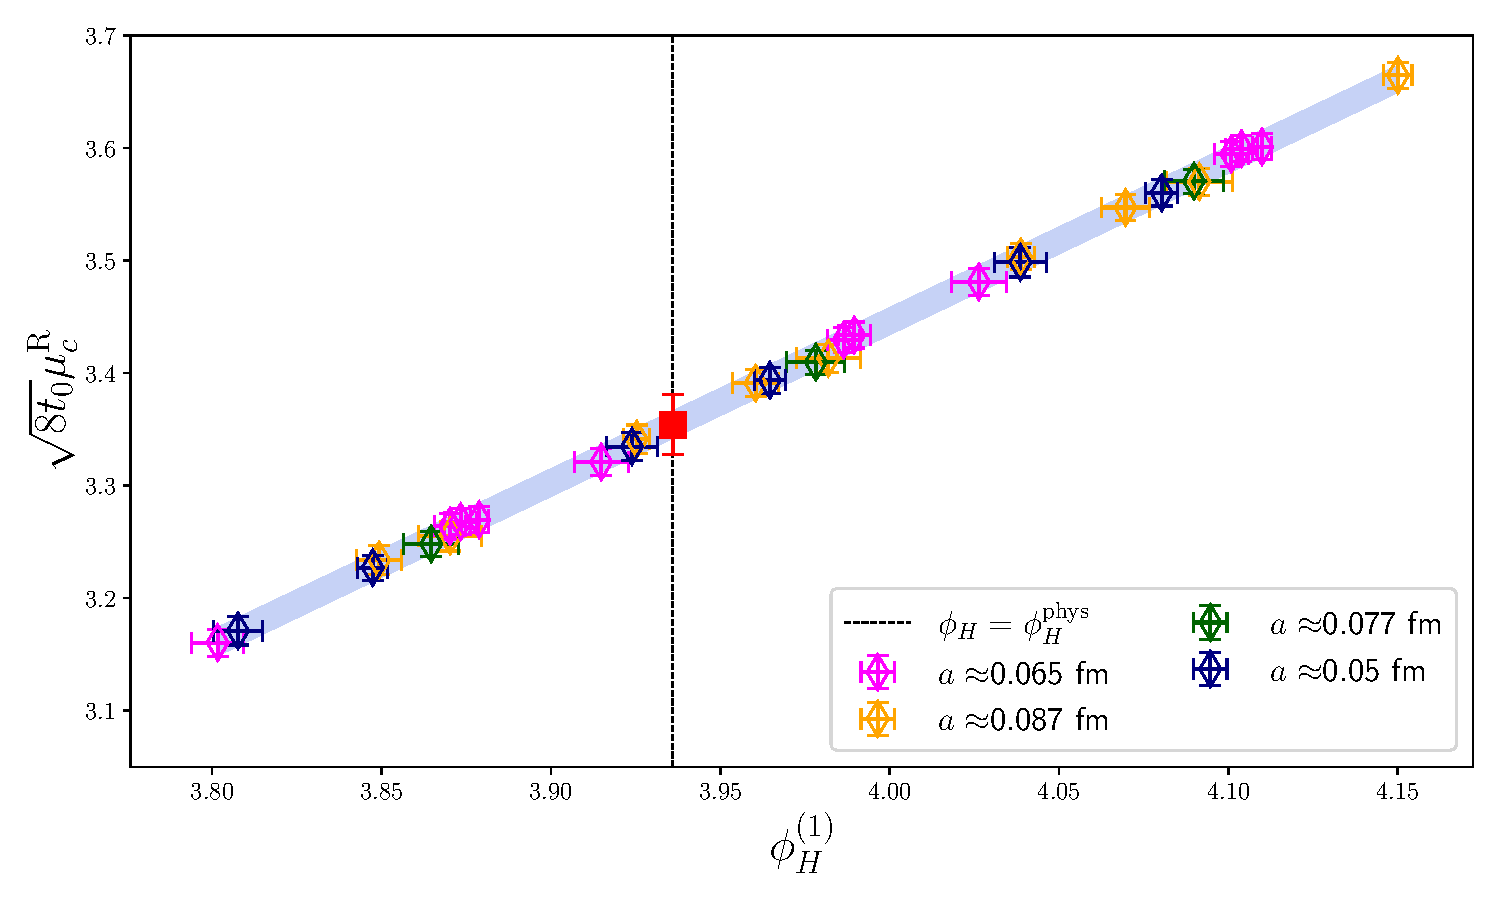
\includegraphics[scale=0.50]{./cap6/figs/mc/fit_phih_interp_muc_fl_ave.pdf}
 	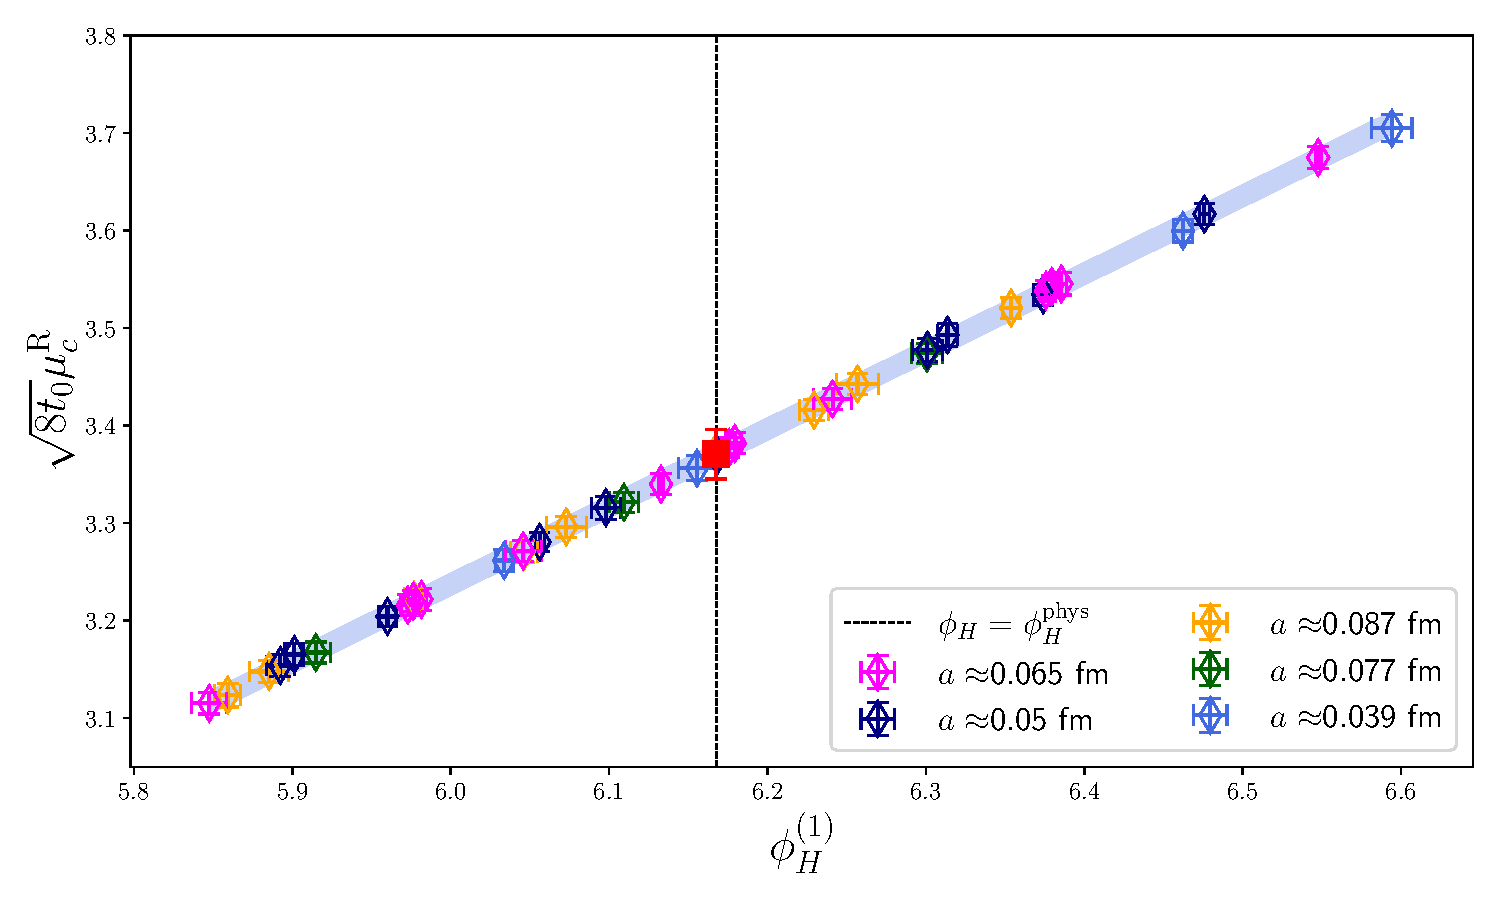
\includegraphics[scale=0.50]{./cap6/figs/mc/fit_phih_interp_muc_etac.pdf}
 	\caption{ Heavy mass dependence of the renormalised charm quark mass $\mu_c^{\rm\scriptscriptstyle R}$ in units of $\sqrt{8t_0}$ for the fits with larger weights according to the TIC criteria. \textit{Top}: Results shown for the flavour-averaged matching condition $\phi_{H}^{(1)} = \sqrt{8t_0} m_{\overline{H}}$. \textit{Bottom}: Results shown for the $\eta_h^{\mathrm{conn}}$ matching condition $\phi_{H}^{(2)} = \sqrt{8t_0} m_{\eta_h}^{\mathrm{conn}}$. Dependencies other than $\phi_H^{(i)}$ in the chiral-continuum extrapolation have been projected to the physical point. The red square symbols indicate the continuum results at the physical value $\phi_H^{\mathrm{phys}}$. We observe a linear dependence of the charm quark mass on the different matching conditions used in this work. }
 	\label{fig:mc_mh_dependence}
 \end{figure}

Regarding the lattice spacing dependence of the charm quark mass, we assume the leading cutoff effects to 
be $O(a^2)$, as discussed above. Corrections of odd order in $a$ are generically expected to be highly
suppressed at maximal twist, by way of the extension of the argument for automatic $O(a)$
improvement; we thus include $a^4$ terms to account for deviations from linear behaviour
in $a^2$. Finally, we allow for terms proportional to $m_\pi^2$ and to various powers of the charm
mass. The generic ansatz to parameterise lattice spacing dependence thus take the following form
\begin{equation}
	c_{\mu_c}(a, \phi_2, \phi_H) = \frac{a^2}{8t_0} \big(
	c_1 + c_2\phi_2 + c_3 \phi_H^2
	\big)
	+
	\frac{a^4}{(8t_0)^2}\big(
	c_4 + c_5\phi_H^2 + c_6 \phi_H^4
	\big).
	\label{eq:lattice_spacing_dependence}
\end{equation} 

In order to estimate the systematic effects arising from the model variation, we consider all the possible 
combinations where some of the $c_i$ coefficients vanish, save for $c_1$ which is always kept.
Furthermore, following~\cite{Heitger:2021apz}, we allow for cutoff effects to enter either linearly or 
non-linearly, viz.,
  \begin{eqnarray} 	\label{eq:tot_model}
 	\sqrt{8t_0}\mu_c^{R,\text{linear}}(a, \phi_2,\phi_H) &=&
 	\sqrt{8t_0}\mu_c^{R,\text{cont}}(0, \phi_2,\phi_H) + c_{\mu_c}(a, \phi_2,\phi_H),
 	\\
 	\sqrt{8t_0}\mu_c^{R,\text{non-lin}}(a, \phi_2,\phi_H) &=& 
 	\sqrt{8t_0}\mu_c^{R,\text{cont}}(0, \phi_2,\phi_H) \big(1+ c_{\mu_c}(a, \phi_2,\phi_H)\big). \nonumber
 \end{eqnarray}
We thus end up with a total of 64 functional forms for each of the two charm matching conditions,
i.e., a total of 128 models.
Fit parameters are estimated minimising an uncorrelated
$\chi^2$ where, however, the covariance between the independent variables and the data is taken into account. As previously discussed, the goodness-of-fit of fit can still be obtained in this case from the measurement of the $\chi^2_{\mathrm{exp}}$ and the associated p-value. The TIC result for each model is then fed into the model averaging procedure summarised in App.~\ref{app:TIC},
which finally allows to quote a systematic uncertainty that reflects the fluctuations
engendered by the variety of fit ansaetze.

In Table \ref{tab:mc_results_all_matching} we report the results for $\mu_c^{\rm\scriptscriptstyle R}$
in units of $\sqrt{8t_0}$ obtained with each of the two matching conditions independently,
as well as for the combined model average.  

In Figure~\ref{fig:mc_model_av_summary} we summarise the model average procedure, showing some of the best  
fit results coming from the functional forms defined in Eq.~(\ref{eq:tot_model}) for the two
 matching 
conditions studied in this work. Each circle corresponds to a result coming from  a particular model, and 
the opacity is associated to its weight determined from our Takeuchi's Information Criterion (TIC)  as explained in App.~\ref{app:TIC}.  We observe that for both
matching conditions the majority of the models with relevant weights nicely agree, and as a result the 
systematic error is subleading with respect to the statistical uncertainty. Figure~\ref{fig:mc_histogram}  shows a weighted histogram of our results 
coming from different fits. We observe that models cluster mainly around two values, which are adequately
covered by our quoted systematic uncertainty. 


\begin{table}[t!]
	\begin{center}	
		\begin{tabular}{c ||  c c  c  }
			\hline
			 &  $\phi_{H}^{(1)}$ & $\phi_{H}^{(2)} $  &   \text{combined} \\ [0.5ex]
			\hline\hline
			$\sqrt{8t_0}\mu_c^{\rm\scriptscriptstyle R}$ & 3.354(28)(6) & 3.363(27)(6)  &   3.361(26)(7)   
		\end{tabular}
		\caption{Results of the model average for the renormalised charm quark mass  in units of $\sqrt{8t_0}$ based on the two
		 charm quark mass matching conditions --- $\phi_H^{(1)}$ denotes the flavour-averaged matching 
		 condition in \req{eq:fl_av_matching} and  $\phi_H^{(2)}$ the $\eta_h^{\mathrm{conn}}$ matching prescription in 
		 \req{eq:etac_matching}. The last column reports the combined result from these two matching procedures according to our model average prescription. The first error is 
		 statistical, while the second is the systematic uncertainty arising from the model variation.
                }
		\label{tab:mc_results_all_matching}
	\end{center}
\end{table}


\begin{figure}[!htb]
	\centering
	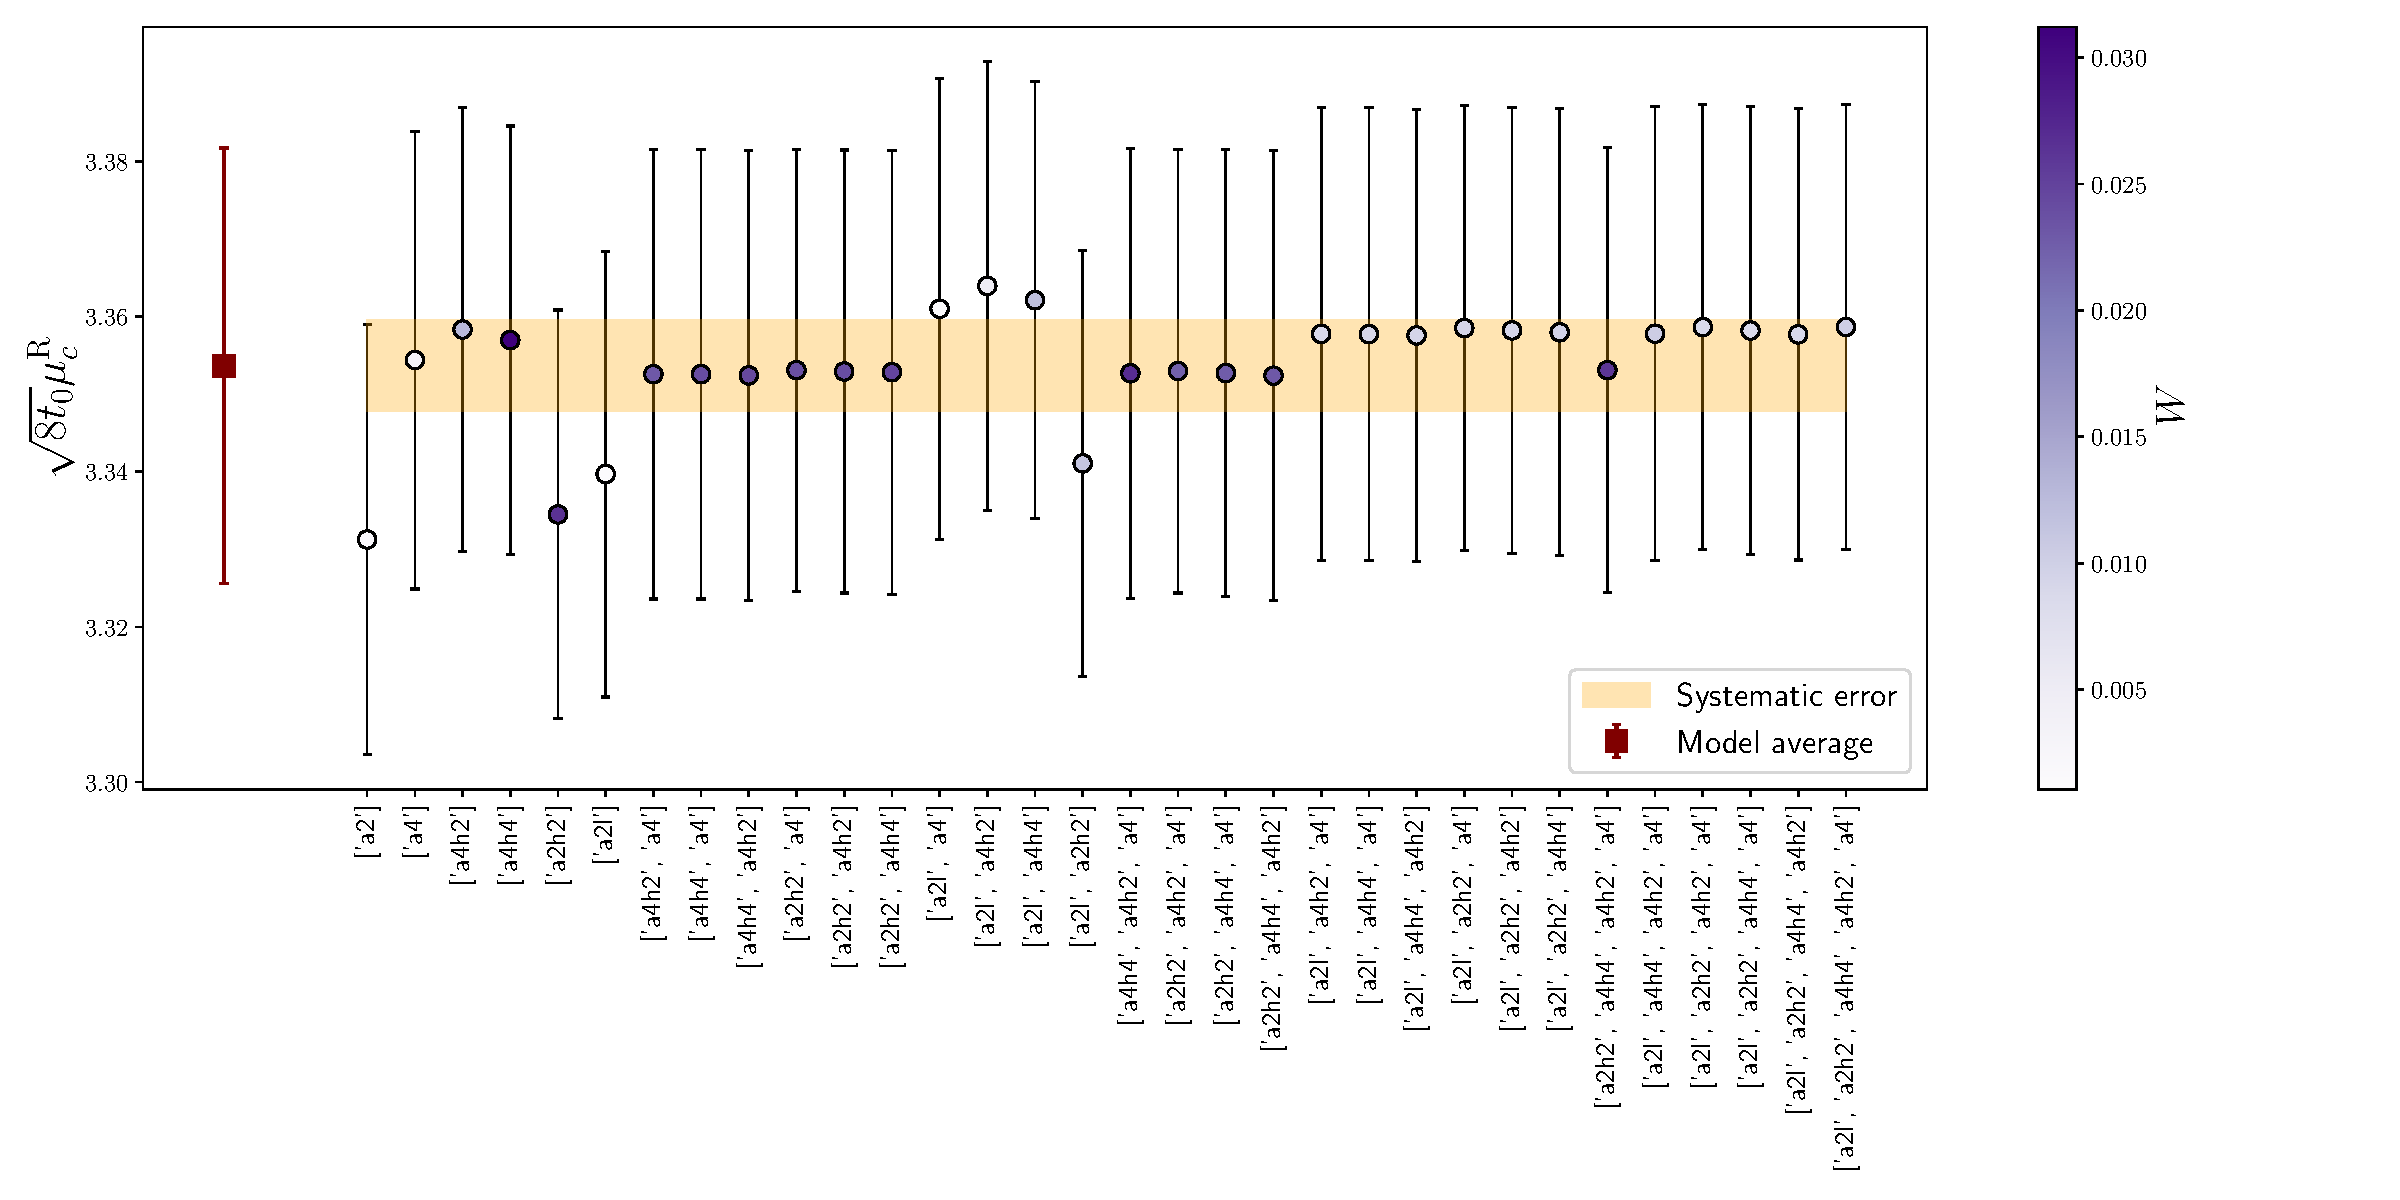
\includegraphics[scale=0.42]{./cap6/figs/mc/cat_ave_tot_muc_fl_ave.pdf}
	\caption{Model average procedure for the renormalised charm quark mass $\mu_c^{\rm\scriptscriptstyle R}$ in units of $\sqrt{8t_0}$. We collect a subset of the best results according to the TIC procedure, coming from different models, for the flavour-averaged  matching condition $\phi_H^{(1)}$.   The opacity of each circle data point reflects the associated normalised weights $W$ as given from the TIC. The yellow shaded band represents the systematic error computed with Eq.~(\ref{eq:weighted_variance}), while the left-most red square symbol corresponds to the result extracted from the model average procedure. The labels of the 32 models specified in the horizontal axis are related to the terms appearing in Eq.~(\ref{eq:lattice_spacing_dependence}) -- characterising the lattice spacing dependence -- in the following way: \texttt{`a2'} corresponds to the term depending on the fit parameter $c_1$. Similarly, \texttt{`a2l', `a2h2', `a4', `a4h2', `a4h4'} refer to $c_2,\dots, c_6$, respectively. Given that the parameter $c_1$ is included in all the models, the associated label is not explicitly specified for all cases appearing in the horizontal axis.}
	\label{fig:mc_model_av_summary}
\end{figure}

\begin{figure}[!htb]
	\centering
	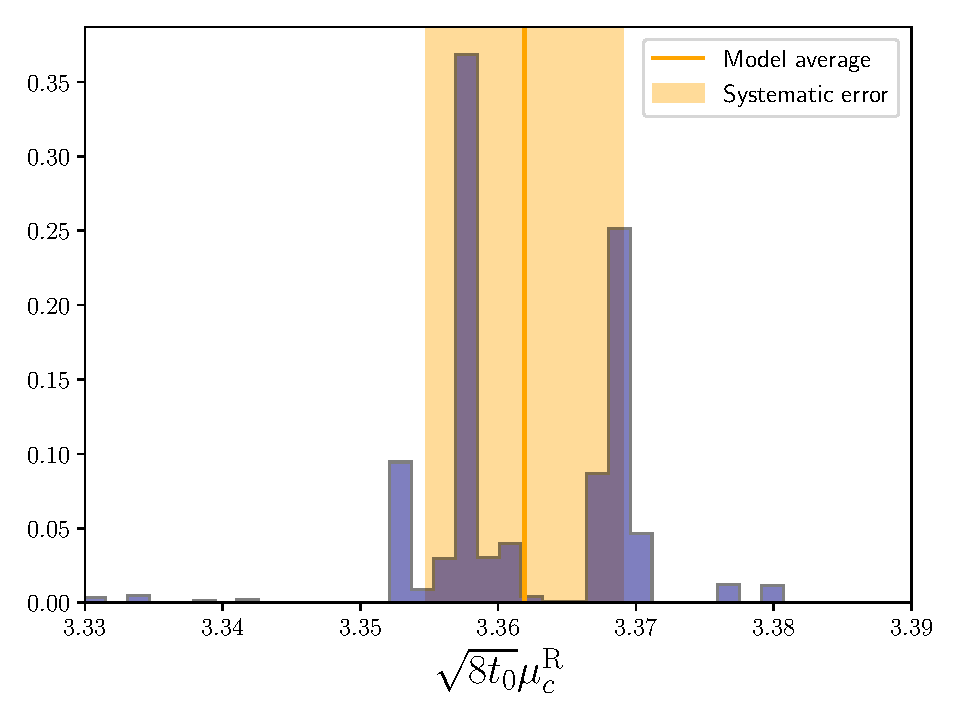
\includegraphics[scale=0.65]{./cap6/figs/mc/hist_muc.pdf}
	\caption{Weighted histogram illustrating the model average procedure for $\sqrt{8t_0}\,\mu_c^{\rm\scriptscriptstyle R}$. The result from each of the 128 models -- including both matching conditions $\phi_H^{(1)}$ and $\phi_H^{(2)}$ -- parameterising the lattice spacing dependence is weighted by its normalised weight $W$ based on the TIC. The vertical line represents the central value from the model average, while the vertical band shows the corresponding estimate of the systematic error.            }
	\label{fig:mc_histogram}
\end{figure}

Figure~\ref{fig:mc_continuum_limit} illustrates typical fits for each of the matching conditions, chosen 
among those with higher weights according to the TIC prescription. The plot shows  the continuum limit behaviour of 
the charm quark mass in units of $\sqrt{8t_0}$. Results coming from the two matching strategies perfectly 
agree in the continuum, in spite of displaying a qualitatively different structure in cutoff effects.
We observe a scaling of the charm quark mass in reasonable
agreement with the $O(a^2)$ leading order, confirming the automatic $O(a)$-improvement of our setup;
nevertheless, we notice that given the current statistical accuracy, fits with  $O(a^4)$ terms are the 
preferred ones from the model average, since they allow to properly describe the curvature in our data. 
Note also the overall small size of scaling violations, which are at the few percent level.
Finally, Figure~\ref{fig:mc_pion_dependence} shows the pion  mass dependence of the charm quark mass. As 
expected, we observe a mild dependence of the charm mass on the light quark masses.
 
\begin{figure}[!htb]
	\centering 
	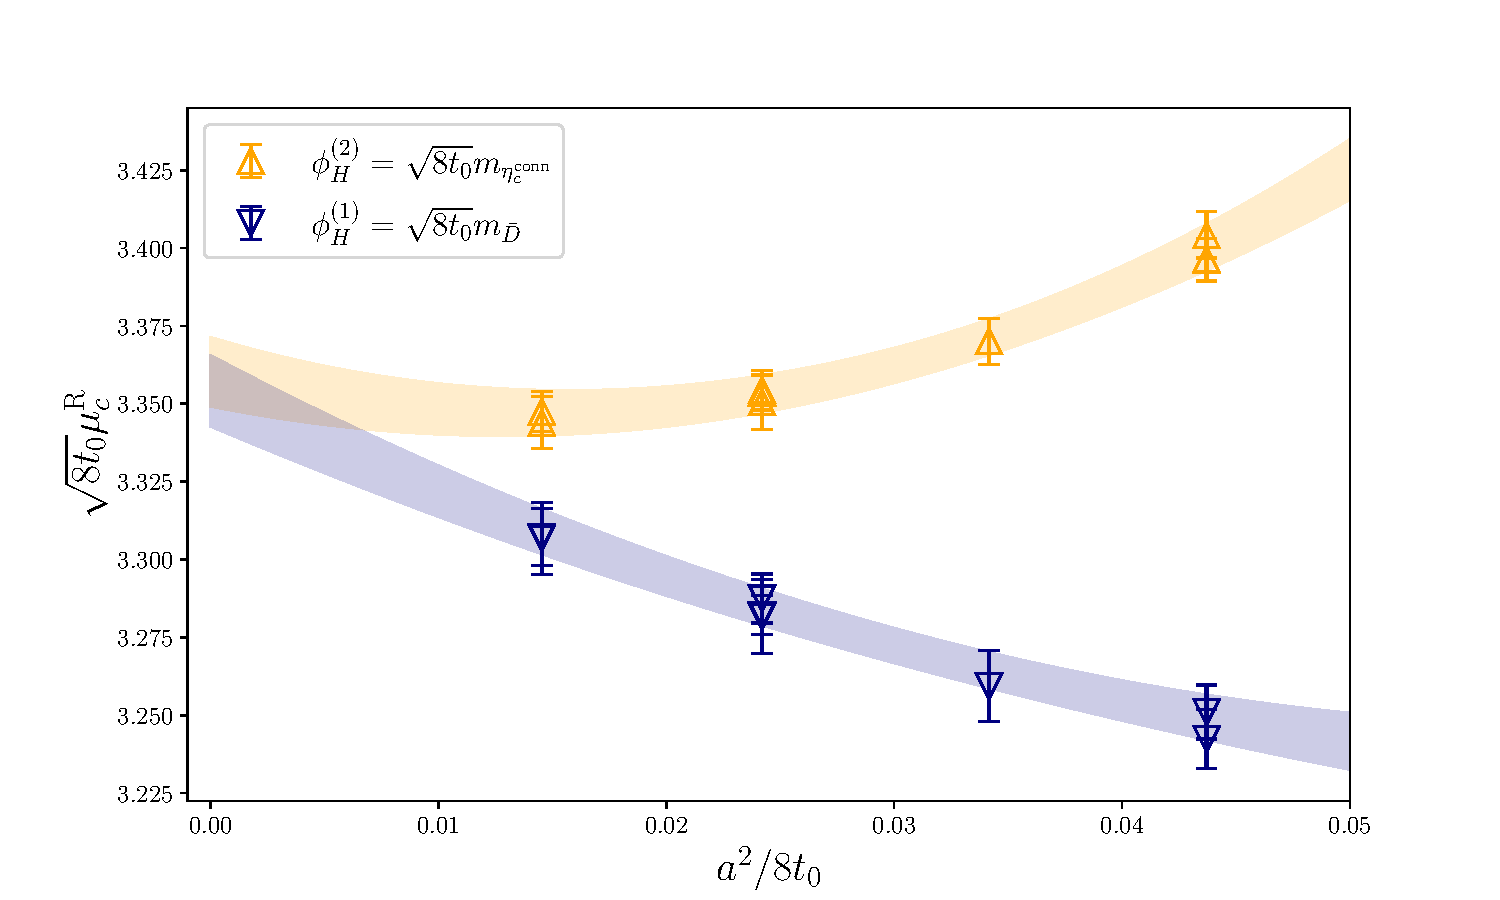
\includegraphics[scale=0.6]{./cap6/figs/mc/mc_cl_all_cat.pdf}
	\caption{Comparison of the continuum limit approach for the two  charm matching 
	prescriptions. Shown are two of the fits with highest weights from the TIC, projected onto the lattice 
	spacing dimension. In yellow we show results for the $\eta_h^{\mathrm{conn}}$ matching condition, while  the blue 
	points illustrate  the flavour-averaged matching. Each data-point in this plot is projected to the 
	physical pion mass and the physical charm quark mass, in order to properly visualise the lattice 
	spacing dependence. }
	\label{fig:mc_continuum_limit}
\end{figure}

\begin{figure}
	\centering
	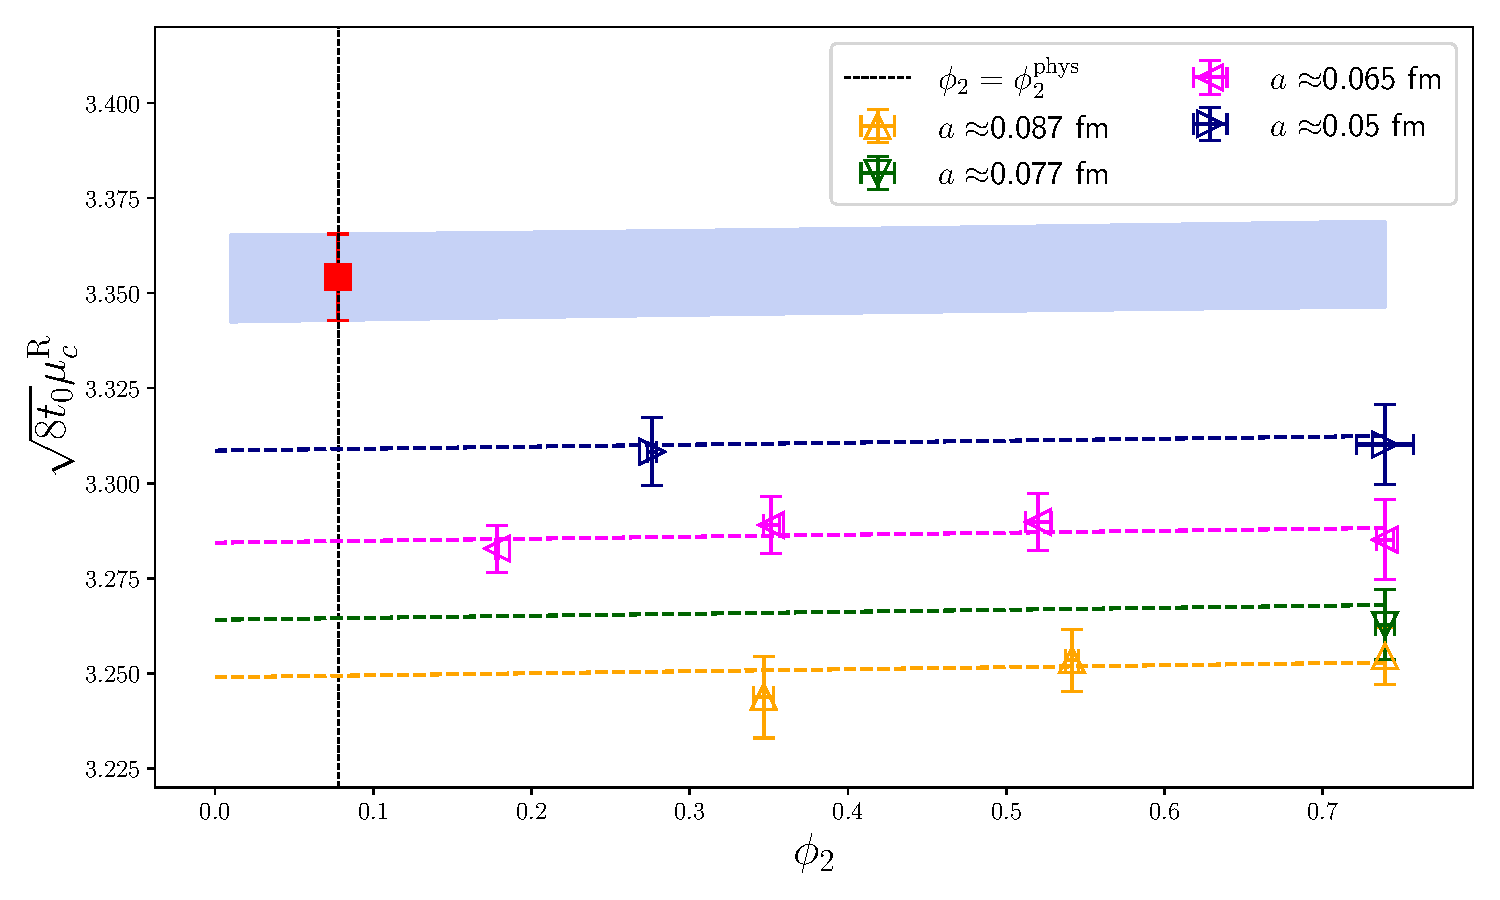
\includegraphics[scale=0.52]{./cap6/figs/mc/fit_phi2_muc_fl_ave.pdf}
	\caption{Pion mass dependence of the charm quark mass for one of the best  fits according to the TIC criteria. Results are shown for the flavour-averaged matching condition. Each point corresponds to the  value for a given ensemble, projected to the physical charm quark mass. The dashed lines represent the chiral trajectories at finite lattice spacing, while the blue shaded band is a projection to the continuum limit. The red point shows our final result extrapolated at the physical point in the continuum. }
	\label{fig:mc_pion_dependence}
\end{figure}


\subsection{Results for the charm quark mass}

The renormalised charm quark mass 
$\mu_c^{\rm\scriptscriptstyle R}$ can be obtained once we combine the results collected in Table~\ref{tab:mc_results_all_matching} with our determination of $\sqrt{t_0^{\mathrm{phys}}}$ in Eq.~(\ref{eq:t0phys}). As discussed at the beginning of this section, the knowledge of the renormalisation group running factors allows  to quote
results for the RGI and $\MSbar$ values of the charm quark mass.

After combining the results from our 128 fitting models through the model average procedure,
and using the running factor in \req{eq:rgi_running_factor}, we quote for the three-flavour theory
the value for the RGI quark mass
\begin{eqnarray}
  M_c^{\mathrm{RGI}}(\NF=3) &=& 1.485(8)(3)(14)[17]\ \mathrm{GeV}\,,
	\label{eq:rgi_charm_mass_result}
\end{eqnarray}
where the first error is statistical, including the uncertainty on  $t_0^{\mathrm{phys}}$,  the second accounts for the systematic uncertainty, derived from the model average, the third is the error contribution from the RGI running factor in Eq.~(\ref{eq:rgi_running_factor}), and the last error in brackets is the total uncertainty. 

Figure~\ref{fig:mc_error_contributions} illustrates the relative contribution of various sources of error to the
uncertainty of our determination of $M_c^{\mathrm{RGI}}$. The dominant source of error comes from the 
renormalisation group running of Eq.~(\ref{eq:rgi_running_factor}), while the second most relevant 
contribution arises from the statistical error of  the correlation functions computed in each ensembles.  
The  error coming from  the uncertainty on $t_0^{\mathrm{phys}}$ based on our  scale setting  procedure~\cite{MA1}, as well as the 
systematic error from the model average  are subleading contributions. We therefore expect
that the 
inclusion in this charm quark mass analysis of further ensembles -- with finer lattice spacings and at physical pion masses --  will only have a significant impact if combined with improved determinations of the RGI running factor and the scale setting procedure.
%
\begin{figure}[t!]
	\centering
	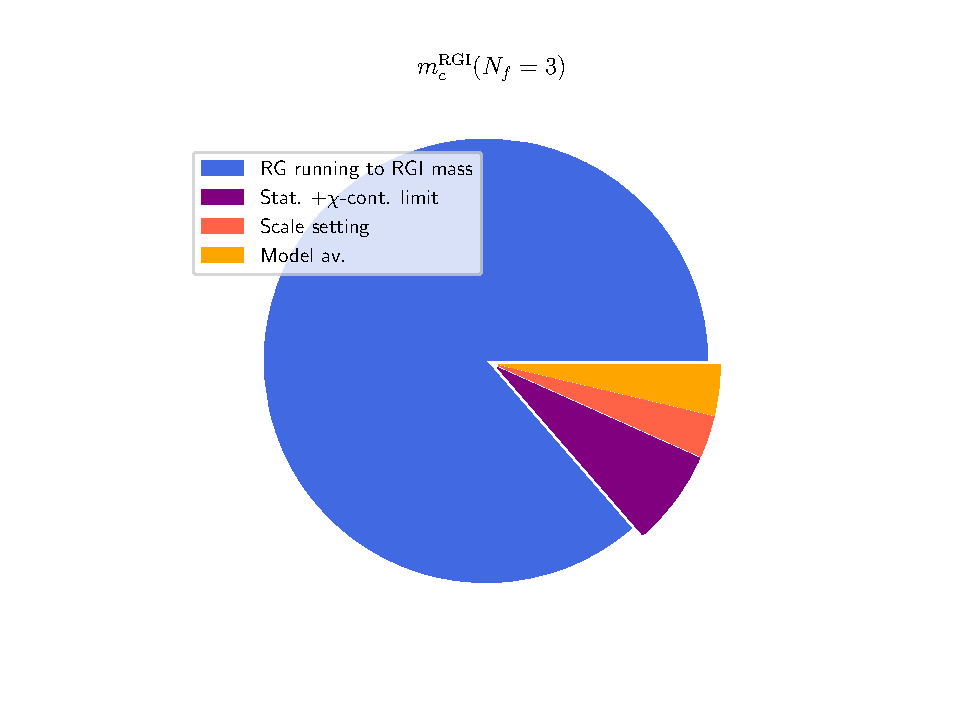
\includegraphics[scale=0.7]{./cap6/figs/mc/mc_error_pie.pdf}
	\caption{Relative contributions to the total variance of our final result for $M_c^{\mathrm{RGI}}$. The dominant piece comes from the error in the non-perturbative determination of the renormalisation group running factor to the RGI mass quoted in Eq.~(\ref{eq:rgi_running_factor}). The label statistical plus $\chi$-continuum limit stands for the error arising from the statistical accuracy of our data and the chiral-continuum extrapolation, while the scale setting piece comes from the physical value of the gradient flow scale $t_0^{\mathrm{phys}}$. Finally, the model average piece illustrates the systematic error arising from the set of models considered in this work.
          }
	\label{fig:mc_error_contributions}
\end{figure}
%


In order to quote results in the $\MSbar$ scheme, we use five-loop perturbation theory for the quark
mass anomalous dimension~\cite{Baikov:2014qja,Luthe:2016xec,Baikov:2017ujl} and the beta function~\cite{Baikov:2016tgj,Herzog:2017ohr,Luthe:2017ttc}.
The matching between the $\NF=3$ and $\NF=4$ theories uses the four-loop decoupling effects~\cite{Liu:2015fxa}
incorporated into the RunDec package~\cite{Chetyrkin:2000yt,Schmidt:2012az,Herren:2017osy}. Renormalisation group equations are solved using as input the value 
$\Lambda^{(3)}_{\overline{\mathrm{MS}}} = 341(12)\ \mathrm{MeV}$ from~\cite{Bruno:2017gxd}. The correlation arising from the fact that a common subset of gauge field configuration ensembles were employed in the computation of $\Lambda^{(3)}_{\overline{\mathrm{MS}}}$ and the non-perturbative running factor in Eq.~(\ref{eq:rgi_running_factor}) is taken into account. We thus arrive to the following results for the RGI and $\MSbar$-scheme charm quark masses in the 4-flavour theory,
\begin{eqnarray}
  M_c^{\mathrm{RGI}}(\NF=4) &=& 1.546(8)(3)(14)(4)_\Lambda(3)_{\rm trunc.}[17] \ \mathrm{GeV}\,,\\
  \overline{m}_c(\mu=3\ \mathrm{GeV}, \NF=4) &=& 1.006(5)(2)(9)(6)_\Lambda(3)_{\rm trunc.}[13] \ \mathrm{GeV}\,,
	\\
	\overline{m}_c(\mu=\overline{m}_c, \NF=4) &=& 1.296(5)(2)(8)(11)_\Lambda(5)_{\rm trunc.}[16] \ \mathrm{GeV}\,,
\end{eqnarray}
where the first and second errors arise from the statistical and systematic errors, respectively, in the value of $M_c^{\mathrm{RGI}}(\NF=3)$ in Eq.~(\ref{eq:rgi_charm_mass_result}), the third error is due to the non-perturbative running factor in Eq.~(\ref{eq:rgi_running_factor}), the fourth error is related to the uncertainty in $\Lambda^{(3)}_{\overline{\mathrm{MS}}}$, the fifth error is an estimate of the truncation uncertainty from the deviation between the 5-loop and 4-loop results, and the last error in brackets is the total error. We observe that at the lower renormalisation scale, $\mu=\overline{m}_c$, the scale invariant $\MSbar$ charm mass, $\overline{m}_c(\mu=\overline{m}_c, \NF=4)$, receives a large contribution to its error from the uncertainty of $\Lambda^{(3)}_{\overline{\mathrm{MS}}}$ and from the truncation error. These specific sources of uncertainty are less prominent in the RGI mass, $M_c^{\mathrm{RGI}}(\NF=4)$.

In Figure~\ref{fig:mc_comparison} we compare our determinations of the charm quark mass in the $\MSbar$ scheme with the results from other lattice QCD calculations also based on $\NF=2+1$ dynamical simulations and with the corresponding FLAG average~\cite{FlavourLatticeAveragingGroupFLAG:2021npn}. We observe in particular a good agreement with the results from \cite{Heitger:2021apz} which are also based on CLS ensembles but employ Wilson fermions in the valence sector.

\begin{figure}[t!]
	\centering
	\hspace{-0mm}
	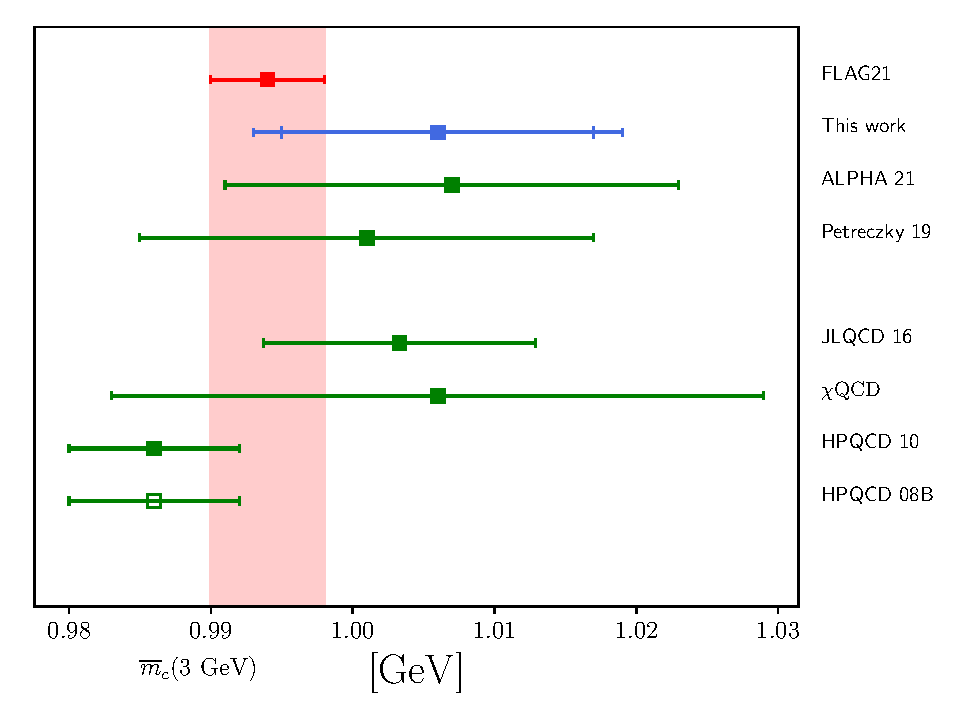
\includegraphics[scale=0.47]{./cap6/figs/mc/mc_comparison_3gev.pdf}
	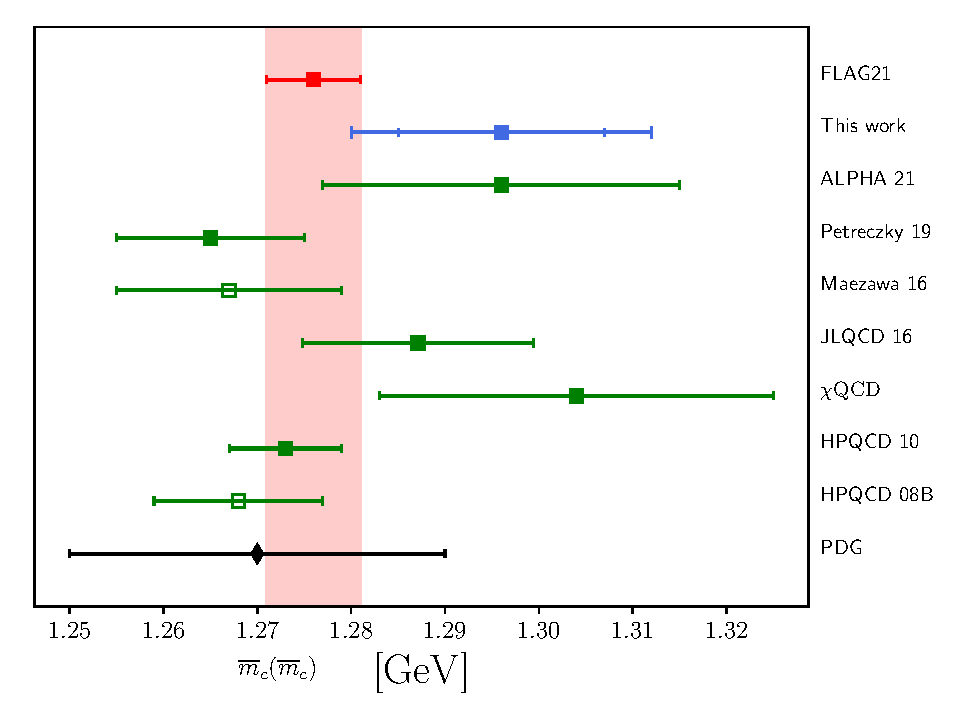
\includegraphics[scale=0.47]{./cap6/figs/mc/mc_comparison.pdf}
	\caption{Comparison of our charm quark mass determinations in the $\MSbar$ scheme with the FLAG average~\cite{FlavourLatticeAveragingGroupFLAG:2021npn} and the results from other lattice QCD calculations based on $\NF=2+1$ dynamical simulations. In our results, shown in blue, we indicate both the total uncertainty and the error when excluding the uncertainty arising from $\Lambda^{(3)}_{\overline{\mathrm{MS}}}$. \textit{Left}: comparison for the  $\overline{m}_c(\mu=3\ \mathrm{GeV}, \NF=4)$. \textit{Right}: comparison for $\overline{m}_c(\mu=\overline{m}_c, \NF=4)$.  Starting from the bottom, results are taken from: PDG \cite{ParticleDataGroup:2022pth}, HPQCD 08B \cite{HPQCD:2008kxl}, HPQCD 10 \cite{McNeile:2010ji}, $\chi$QCD \cite{Yang:2014sea}, JLQCD 16 \cite{Nakayama:2016atf}, Maezawa 16 \cite{Maezawa:2016vgv}, Petreczky 19 \cite{Petreczky:2019ozv}, ALPHA 21 \cite{Heitger:2021apz}.
       }
	\label{fig:mc_comparison}
\end{figure}

%%%%%%%%%%%%%%%%%%%%%%%%%%%%%%%%%%%%%%%%%%%%%%%%%%%%%%%%%%%
%%%%%%%%%%%%%%%%%%%%%%%%%%%%%%%%%%%%%%%%%%%%%%%%%%%%%%%%%%%
%%%%%%%%%%%%%%%%%%%%%%%%%%%%%%%%%%%%%%%%%%%%%%%%%%%%%%%%%%%
%%%%%%%%%%%%%%%%%%%%%%%%%%%%%%%%%%%%%%%%%%%%%%%%%%%%%%%%%%%


\section{Determination of decay constants of charmed mesons}
\label{sec:fDs}

\subsection{Computation of decay constants}

Along with the charm quark mass, in this paper we present a first computation of the $D_{(s)}$
meson decay constants within our setup. In the absence of electromagnetic interactions, the
decay constant fully determines the leptonic decay amplitude of flavoured pseudoscalar mesons,
and is given by the matrix element of the axial current as 
\begin{equation}
	\big| \langle 0 | A_0^{qr} | P^{qr}(\mathbf{p=0})\rangle\big| = \frac{f_{qr} m_{\rm\scriptscriptstyle PS}}{\sqrt{2m_{\rm\scriptscriptstyle PS}L^3}},
	\label{eq:decay_constant_definition}
\end{equation}
where the state $|P^{qr}\rangle$ is the ground state for a pseudoscalar meson with flavour content $qr$,
and $m_{\rm\scriptscriptstyle PS}$ its mass.
The factor $1/\sqrt{2m_{\rm\scriptscriptstyle PS}L^3}$ comes from the usual relativistic normalisation
of one-particle states in finite volume.

With Wilson fermions, the computation of the above matrix elements requires the finite current
normalisation factor $\ZA$ and, if $O(a)$ effects are to be subtracted, a number of improvement
coefficients. With our fully twisted valence sector this is completely bypassed: when $qr$ belong
in a twisted quark doublet --- i.e., have different signs in the twisted mass matrix in \req{eq:mval} ---
the physical axial current, expressed in twisted quark variables, becomes a vector current,
and the Ward identity in \req{eq:vector_ward_id} allows to obtain it from the pseudoscalar
two-point function.
The resulting expression of the correctly normalised pseudoscalar decay constant reads
\begin{equation}
	f_{PS} = \sqrt{\frac{2L^3}{m_{PS}^3}} (\mu_q+\mu_r) | \langle 0 | P^{qr} | P^{qr}(\mathbf{p=0})\rangle |
	\label{eq:renormalised_decay_constant}.
\end{equation}
We will extract the matrix element $ \langle 0 | P^{qr} | P^{qr}(\mathbf{p=0})\rangle $  from the 
normalised eigenvector $v_n(t,t_0)$ of the GEVP  according to \req{eq:effective_matrix_element}. In 
order to extract the large time plateau where excited state contributions are suppressed we perform 
several fits to constant behaviour by varying the fit ranges,
and we assign a weight to each fit by means of the TIC prescription as
described in App.~\ref{app:TIC}. The results  for the ground state 
matrix element are then extracted through the model average given by \req{eq:model_average}.
In Figure  \ref{fig:decay_plateau} we show a representative plateau for a heavy-light decay constant, 
together with a summary of the model average with different fit intervals.


\begin{figure}
	\centering
	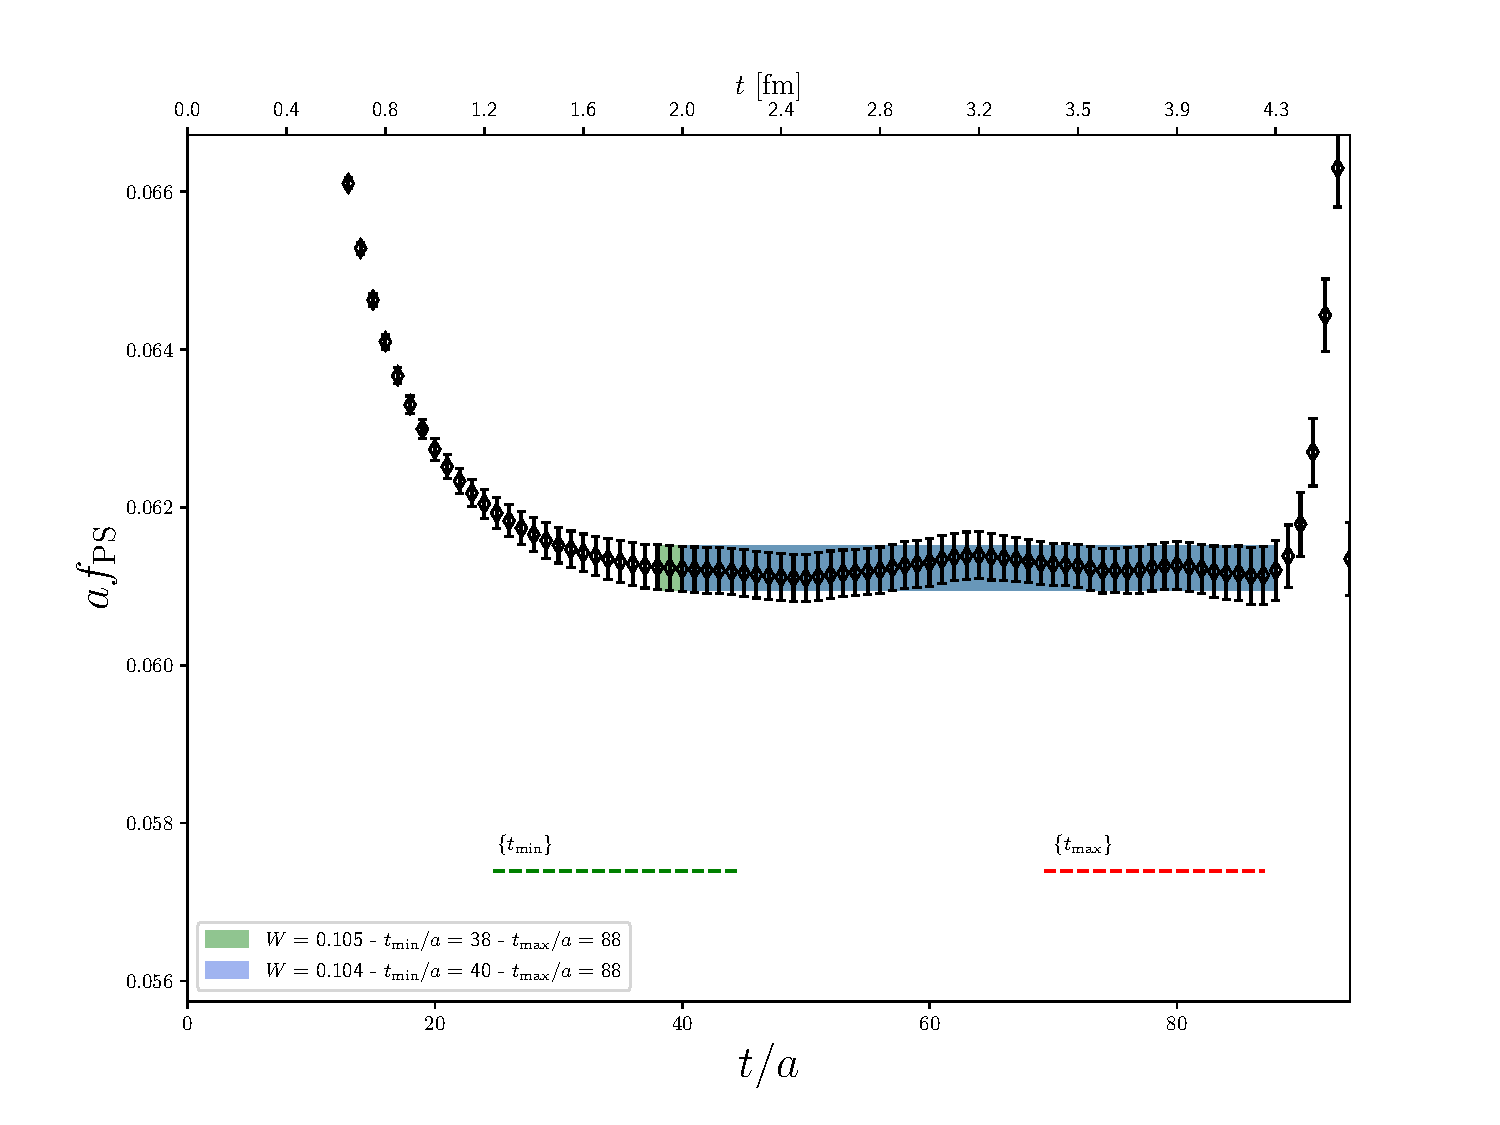
\includegraphics[scale=0.5]{./cap6/figs/fds/f8_plateau.pdf}
	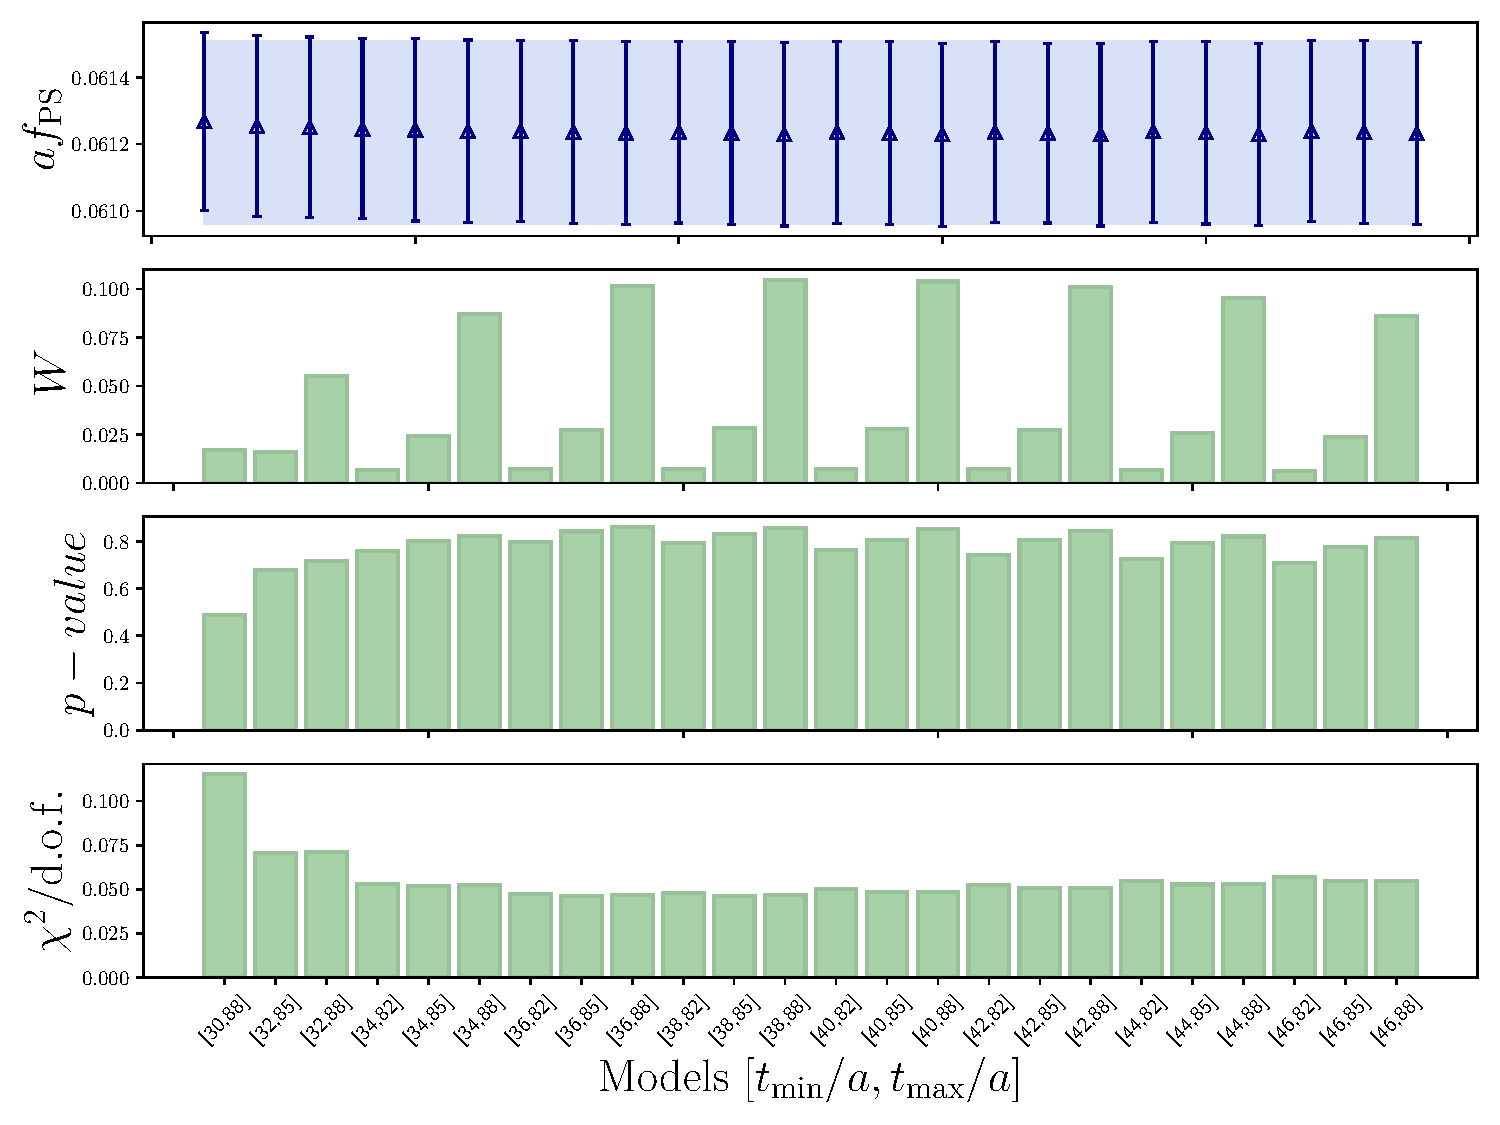
\includegraphics[scale=0.5]{./cap6/figs/fds/f8_BMA.pdf}
	\caption{Illustration of the extraction of the heavy-light pseudoscalar decay constants, after applying a GEVP analysis, for ensemble J303. \textit{Top}: plateau for the heavy-light pseudoscalar decay constant for the two fit intervals with higher weights in the model average. \textit{Bottom}: summary of results from  different fit ranges together with weights $W$, p-values and $\chi^2/d.o.f.$. The shaded blue band represents the model average result. }
	\label{fig:decay_plateau} 
\end{figure}


\subsection{Chiral-continuum fits and results for $f_{D_{(s)}}$}

The chiral-continuum fits for the $D_{(s)}$ meson decay constants are performed similarly to the
ones for the charm quark mass. By exploiting Chiral Perturbation Theory with heavy quarks 
\cite{Grinstein:1992qt, Goity:1992tp} to construct appropriate fit functions, we 
extract the physical point observables trough a global fit of the $f_D$ and $f_{D_s}$ decays,
and estimate the systematic effects by applying the model average procedure based on the TIC.

The quantities we fit to are combinations of meson masses and decay constants of the form
\begin{equation}
  \Phi_{D_{(s)}} = (8t_0)^{3/4}f_{D_{(s)}} \sqrt{m_{D_{(s)}}},
  \label{eq:defphiD}
\end{equation}
for which a Heavy Quark Effective Theory (HQET) scaling law in powers of the inverse
heavy quark mass exists.
The general continuum heavy and light quark mass dependence can be expressed as the product of the individual contributions to arrive at the generic expression 
\begin{equation}
	\Phi_{D_{(s)}} = \Phi_{\chi} \left[
	1 + \delta\Phi_{\chi\mathrm{PT}}^{D_{(s)}}
	\right]
	\left[
	1 + \delta\Phi_a^{D_{(s)}}
	\right]\,.
	\label{eq:fds_different_pieces}
\end{equation}
Here $\Phi_\chi$ governs the heavy-quark mass dependence while  $\delta\Phi_{\chi\mathrm{PT}}^{D_{(s)}}$ controls the light quark behaviour as approaching the physical point. Finally the lattice spacing dependence describing cut-off effects is regulated by $\delta\Phi_a^{D_{(s)}}$. In the following, we analyse these terms independently to arrive at a final expression for the $\Phi_{D_{(s)}}$ approach to the physical point.

The continuum heavy-quark mass dependence, $\Phi_\chi$, admits an expression in HQET of the form
\begin{align}
	\Phi_{\chi} = C_{\mathrm{HQET}}(m_h)\, \Phi_0 \left[ 1 + p_h^{(1)} \frac{1}{\phi_H} + p_h^{(2)} \left( \frac{1}{\phi_H} \right)^2 + \dots \right]
	\,,
	\label{eq:phichi}
\end{align}
where $\phi_H=\sqrt{8t_0}m_H$ monitors the heavy quark mass dependence with $m_H$ being the flavour-
average $m_{\bar{H}}$ or the $\eta_h^{\mathrm{conn}}$ pseudoscalar meson masses.
In general, this expression is not expected to have high accuracy in the charm mass region,
due to it being at the limit of applicability of HQET. Furthermore, perturbative values
for the matching factor $C_{\mathrm{HQET}}(m_h)$ have notoriously poor convergence behaviour.\footnote{This
is readily observed in the expression for the coefficient in the $\MSbar$ scheme~\cite{Manohar:2000dt,
	Ji:1991pr},  
\begin{equation} % See Eq. (3.83) of \cite{Manohar:2000dt} and Eq. (10) of \cite{Ji:1991pr}
	C_{\mathrm{HQET}}(m_h) = \left[\alpha_s(m_h)\right]^{{\gamma_0}/{2\beta_0}} \left[1 + \frac{\alpha_s(m_h)}{4\pi}
	\left(-\frac{8}{3} + \frac{\gamma_1}{2\beta_0} - \frac{\gamma_0\beta_1}{2\beta_0^2} \right) + {\mathrm{O}}(\alpha_s^2) \right]\,,
	\label{eq:Wilson-coefficient}
\end{equation}
where, for QCD, $\gamma_0 = -4$, $\gamma_1 = -254/9 - 56\pi^2/27 + 20 \NF/9$, while
the perturbative coefficients of the $\beta$ function have their usual values
$\beta_0 = (11 - 2\NF/3)$ and $\beta_1 = (102 - 28\NF/3)$.
}
However, we are {\em not} interested in modelling the heavy quark mass dependence in a wide
region of masses --- we rather want to interpolate to the charm point from the nearby values
of the heavy masses we compute at. Therefore, we will simply take an expression with
the same functional form for the $m_h$ power corrections, and a constant overall coefficient,
as a convenient ansatz for the interpolation part of our fits. In HQET terms, this amounts
to neglecting the small logarithmic dependence on $m_h$ in a short interval of values.

The light quark mass dependence term, following Heavy Meson $\chi$PT (HM$\chi$PT) considerations,
reads~\cite{Goity:1992tp, Bazavov:2017lyh}
\begin{equation}
	\begin{split}
		\delta \Phi_{\chi {\mathrm{PT}}}^{D} =& - \frac{1+3g^2}{64\pi^2 \phi_f^2} \left[ 3 \mathcal{L}_{\pi} + 2 \mathcal{L}_{K} + \frac{1}{3} \mathcal{L}_{\eta} \right] +
		\frac{4  \phi_2 }{\phi_f^2} \left( p_\chi^{(0)} +  p_\chi^{(2)} \frac{\phi_2}{\phi_f^2} + \frac{p_\chi^{(4)}}{\phi_H} \right),
		\\
		\delta \Phi_{\chi {\mathrm{PT}}}^{D_s} =& - \frac{1+3g^2}{64\pi^2 \phi_f^2} \left[ 4 \mathcal{L}_{K} + \frac{4}{3}  \mathcal{L}_{\eta} \right] +
		\frac{8 \left( \phi_4 - \phi_2 \right)} {\phi_f^2} \left( p_\chi^{(0)} +  p_\chi^{(2)} \frac{\phi_2}{\phi_f^2} + \frac{p_\chi^{(4)}}{\phi_H} \right),
		\label{eq:deltaphichis} 
	\end{split}
\end{equation}
where $p_\chi^{(0,1\,\dots)}$ are fit parameters and $g^2$ is the
$H^\ast H \pi$ coupling in the static and chiral limits, here treated as a free fit parameter alongside
$p_\chi^{(i)}$.  In \req{eq:deltaphichis} we introduced  the notation for the chiral logarithm corrections 
\begin{eqnarray}
	\mathcal{L}_\pi &=& \phi_2 \log(\phi_2), 
	\\
	\mathcal{L}_K &=& \bigg(\phi_4 - \frac{1}{2}\phi_2\bigg)\log(\phi_4 - \frac{1}{2}\phi_2), 
	\\
	\mathcal{L}_\eta &= &\bigg(\frac{4}{3}\phi_4 - \phi_2\bigg)\log(\frac{4}{3}\phi_4 - \phi_2).
\end{eqnarray}
Here $\phi_2$ and $\phi_4$ are the usual hadronic combinations introduced  in \req{eq:phi2_and_phi4},
which control the light and strange quark mass dependence. When working at NLO in the chiral expansion, 
the term
$\phi_f$ appearing in \req{eq:deltaphichis}, which introduces the $\chi$PT scale,
is here replaced by the continuum
physical value  of $\sqrt{8 t_0} f_{\pi K}$, as determined from our setup \cite{MA1} at full twist, with $f_{\pi K}$ given by\footnote{We remind the reader that $f_{\pi K}$ is the quantity used to extract the physical scale $t_0^{\mathrm{phys}}$ in our setup.}
\begin{equation}
	f_{\pi K} = \frac{2}{3} \left(
	f_K + \frac{1}{2}f_\pi
	\right).
\end{equation}
Finally, with similar arguments to the one discussed in the case of the charm quark mass,
the lattice spacing dependence $\delta\Phi_a^{D_{(s)}}$ for the observables $\Phi_{D_{(s)}}$ can be 
parameterised as 
\begin{equation}
	\begin{split}
		\delta \Phi_{a}^{D} &= \frac{a^2}{8t_0} \left[ p_a^{(0)} +  \phi_2 \left( p_a^{(1)} + p_a^{(3)} \phi_H^2 \right) +  p_a^{(2)} \phi_H^2   \right] + {\mathrm{O}}(a^4)
		,
		\\
		\delta \Phi_{a}^{D_s} &= \frac{a^2}{8t_0} \left[ p_a^{(0)} + 2 \left( \phi_4 - \phi_2 \right) \left( p_a^{(1)} + p_a^{(3)} \phi_H^2 \right) +  p_a^{(2)} \phi_H^2   \right]  + {\mathrm{O}}(a^4),
		\, \label{eq:phias}
	\end{split}
\end{equation}
where $p_a^{(0,1,2,\dots)}$ are fit parameters. 

To summarise, for the continuum quark mass dependence  of $\Phi_D$ and $\Phi_{D_s}$
we adopt the expressions
\begin{equation}\small
	\begin{split}
		\Phi_D(0,\phi_2, \phi_H)  &= p_0 + \frac{4p_1}{\phi_f^2}\phi_2 + \frac{p_2}{\phi_H}
		-\frac{1+3g^2}{64\pi\phi_f^2}\bigg(
		3\mathcal{L}_\pi + 2 \mathcal{L}_K + \frac{1}{3}\mathcal{L}_\eta  
		\bigg) +
		\frac{4  \phi_2 }{\phi_f^2} \left( p_\chi^{(0)} +  p_\chi^{(2)} \frac{\phi_2}{\phi_f^2} + \frac{p_\chi^{(4)}}{\phi_H} \right),
		\\
		\Phi_{D_s}(0,\phi_2, \phi_H)  &= p_0 + \frac{8p_1(\phi_4-\phi_2)}{\phi_f^2} + \frac{p_2}{\phi_H}
		-\frac{1+3g^2}{64\pi\phi_f^2}\bigg(
		4 \mathcal{L}_K + \frac{4}{3}\mathcal{L}_\eta\bigg)\\
		&\qquad~
	+\frac{8 \left( \phi_4 - \phi_2 \right)} {\phi_f^2} \left( p_\chi^{(0)} +  p_\chi^{(2)} \frac{\phi_2}{\phi_f^2} + \frac{p_\chi^{(4)}}{\phi_H} \right),
	\end{split}
\end{equation}\normalsize
obtained by combining the light and heavy quark dependencies $\delta\Phi_{\chi \mathrm{PT}}$ and $\Phi_\chi$, 
respectively.  
Following \req{eq:fds_different_pieces}, this then leads to the final ansatz for $\Phi_{D_{(s)}}$
of the form
\begin{equation}
	\Phi_{D_{(s)}}(a,\phi_2, \phi_H) = 
	\Phi_{D_{(s)}}(0,\phi_2, \phi_H) \left[ 1   + \delta\Phi_a^{D_{(s)}}\right].
	\label{eq:fds_combined_fit}
\end{equation}
Since many fit parameters are shared between $\Phi_D$ and $\Phi_{D_s}$, we opt for a global fit for 
determining the two quantities. Moreover, at the symmetric point, i.e.,  for those ensembles with 
degenerate light and strange quark masses $\mu_l=\mu_s$, the two decay constant coincide, and
 $\Phi_D=\Phi_{D_s}$. Therefore, a global fit also helps to constrain the parameters at the symmetric 
 point.

Similarly to the case of the charm quark mass, we consider several specific forms of the fit ansatz,
by setting some combination of fit parameters to zero. We furthermore again match the charm scale using
the two different procedures described in Sec.~\ref{sec:charm_basics}. The result is a total
of 57 different models  for each matching condition,
and we use our TIC criterion to extract a systematic uncertainty associated to the variation
within the full set of fits. In this work, our current approach deliberately excludes fits involving cuts in $\beta$ or pion masses, as with the current subset of ensembles they are significantly penalised by the TIC. As we look ahead to future updates with the complete set of ensembles  we will incorporate cuts in the data within our analysis.

In Figure~\ref{fig:chiral_fits_fds} we show the chiral extrapolations for $f_D$ and $f_{D_s}$
with larger weights in the model average.  From our chiral-continuum extrapolations of $\Phi_D$ and $\Phi_{D_s}$, we observe a mild 
dependence on the  choice of the $\phi_H$ used to match the charm scale. Therefore, in the Figures we 
illustrate the flavour-averaged matching condition only. We also notice that $\Phi_D$ shows some 
curvature in $\phi_2$ arising from the chiral logs, while $\Phi_{D_s}$ presents a more linear behaviour 
while approaching the physical point. Figure~\ref{fig:continuum_fits_fds} shows an illustration
of the scaling towards the continuum limit of $\Phi_D$ and $\Phi_{D_{s}}$. We observe that the continuum 
approach is very well described by leading cutoff effects of $O(a^2)$, as expected for our valence action when it is tuned to maximal twist.
%
\begin{figure}
	\centering
	%\hspace{-1.5cm}
	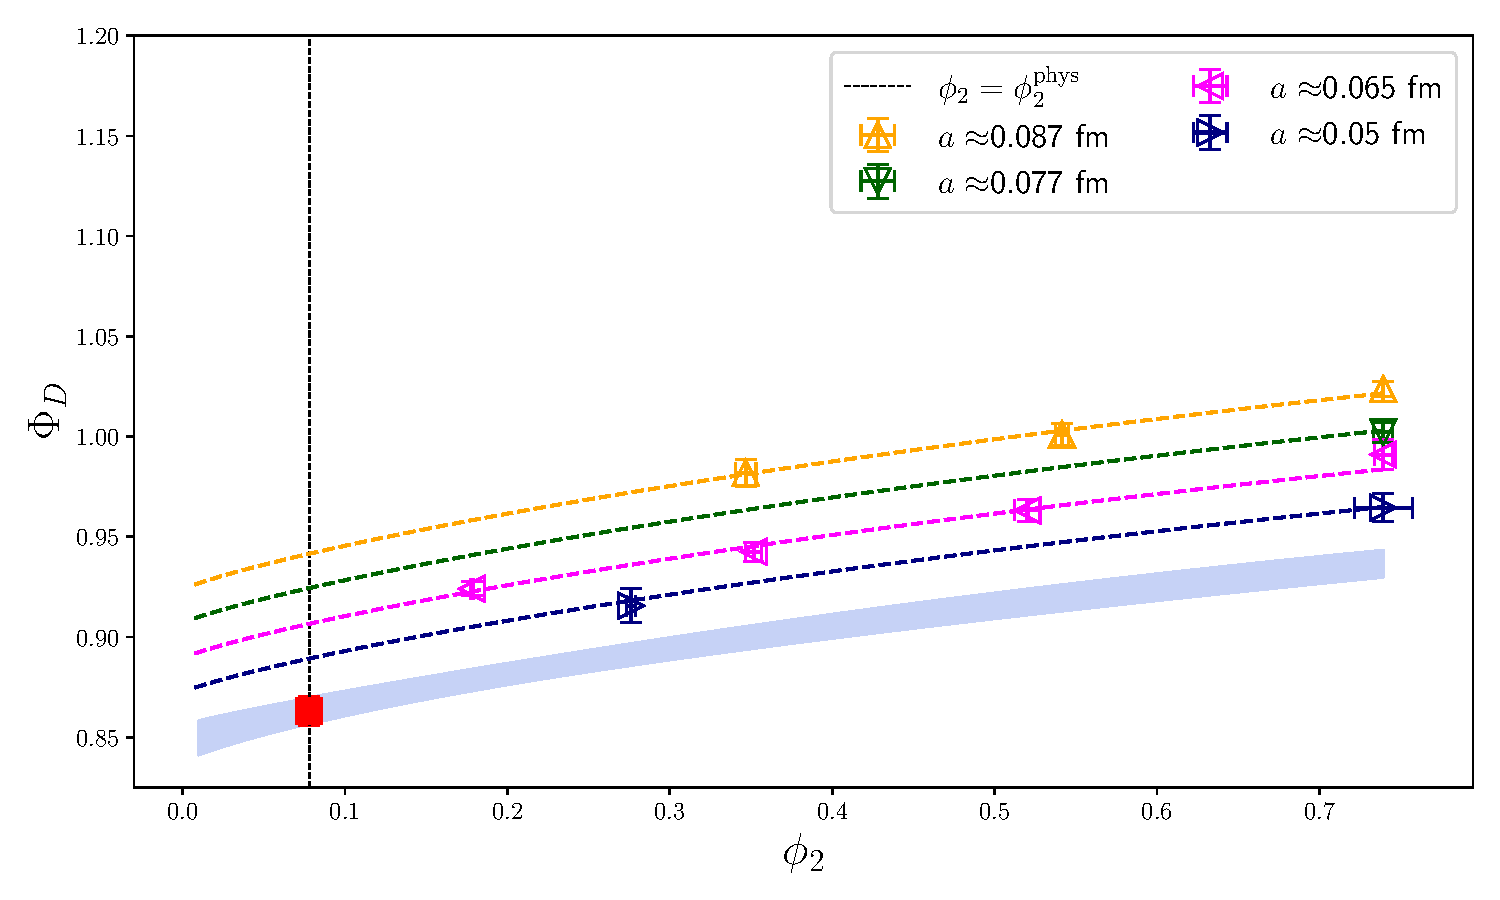
\includegraphics[scale=0.50]{./cap6/figs/fds/fit_fD_fl_ave.pdf}
	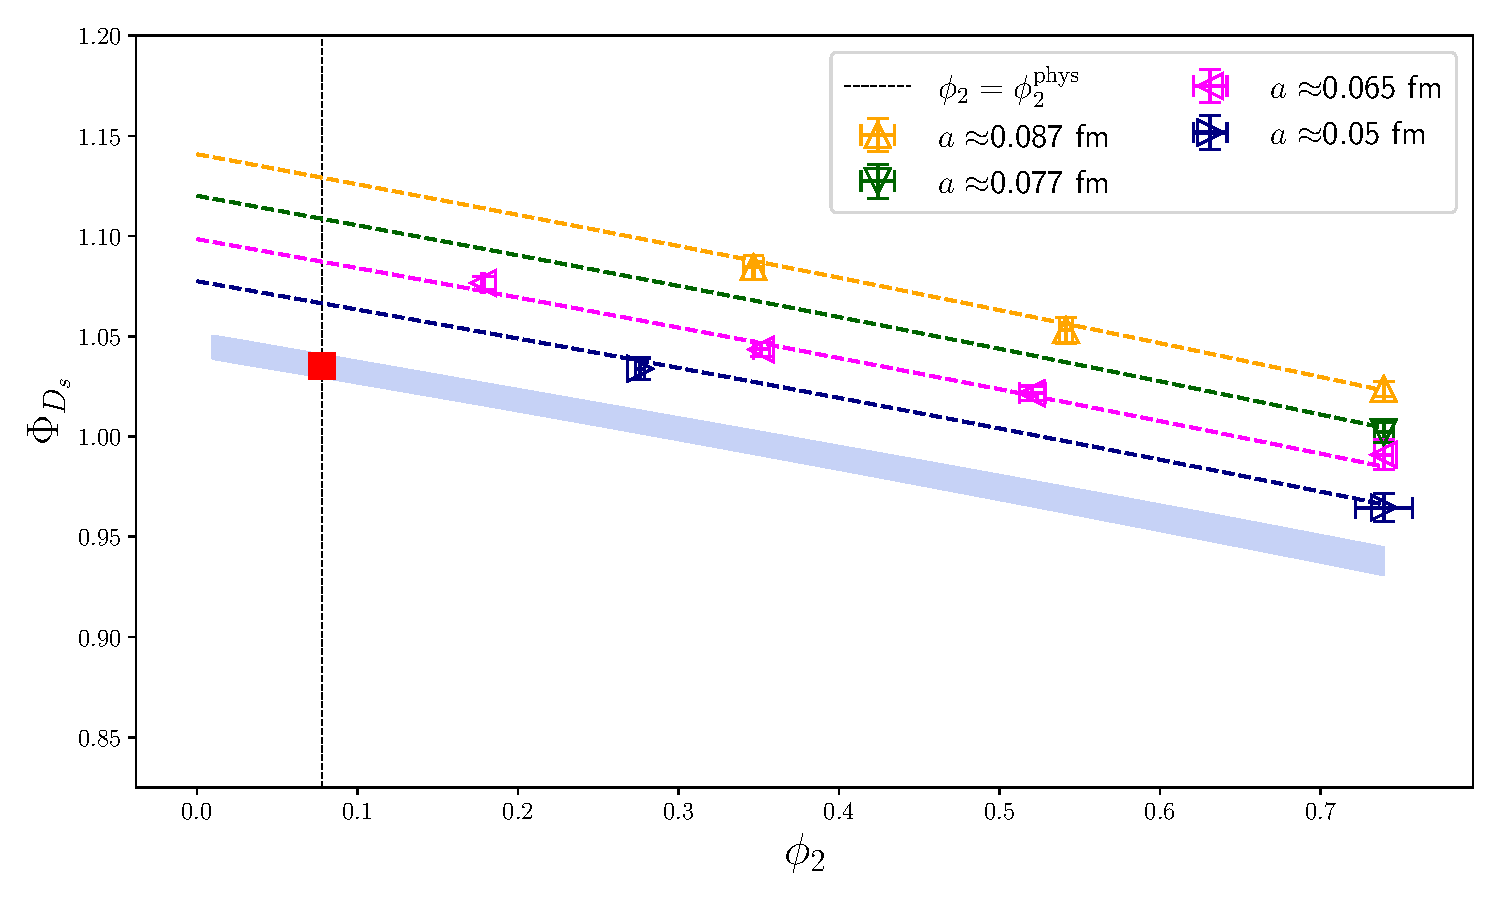
\includegraphics[scale=0.50]{./cap6/figs/fds/fit_fDs_fl_ave.pdf}
	\caption{Chiral behaviour of the best fits according to the TIC criteria applied to  $\Phi_D$ (\textit{top}) and $\Phi_{D_s}$ (\textit{bottom}). Each point is projected to the physical charm quark mass, and results are shown for the flavour-averaged matching condition $\phi_H^{(1)}$. Dashed lines refer to the mass dependence at finite  values of the lattice spacing, while the blue band represents the projection to the continuum limit. Finally, the red square symbols indicate the physical point results.}
	\label{fig:chiral_fits_fds}
\end{figure}

\begin{figure}
	\centering
	%\hspace{-1.5cm}
	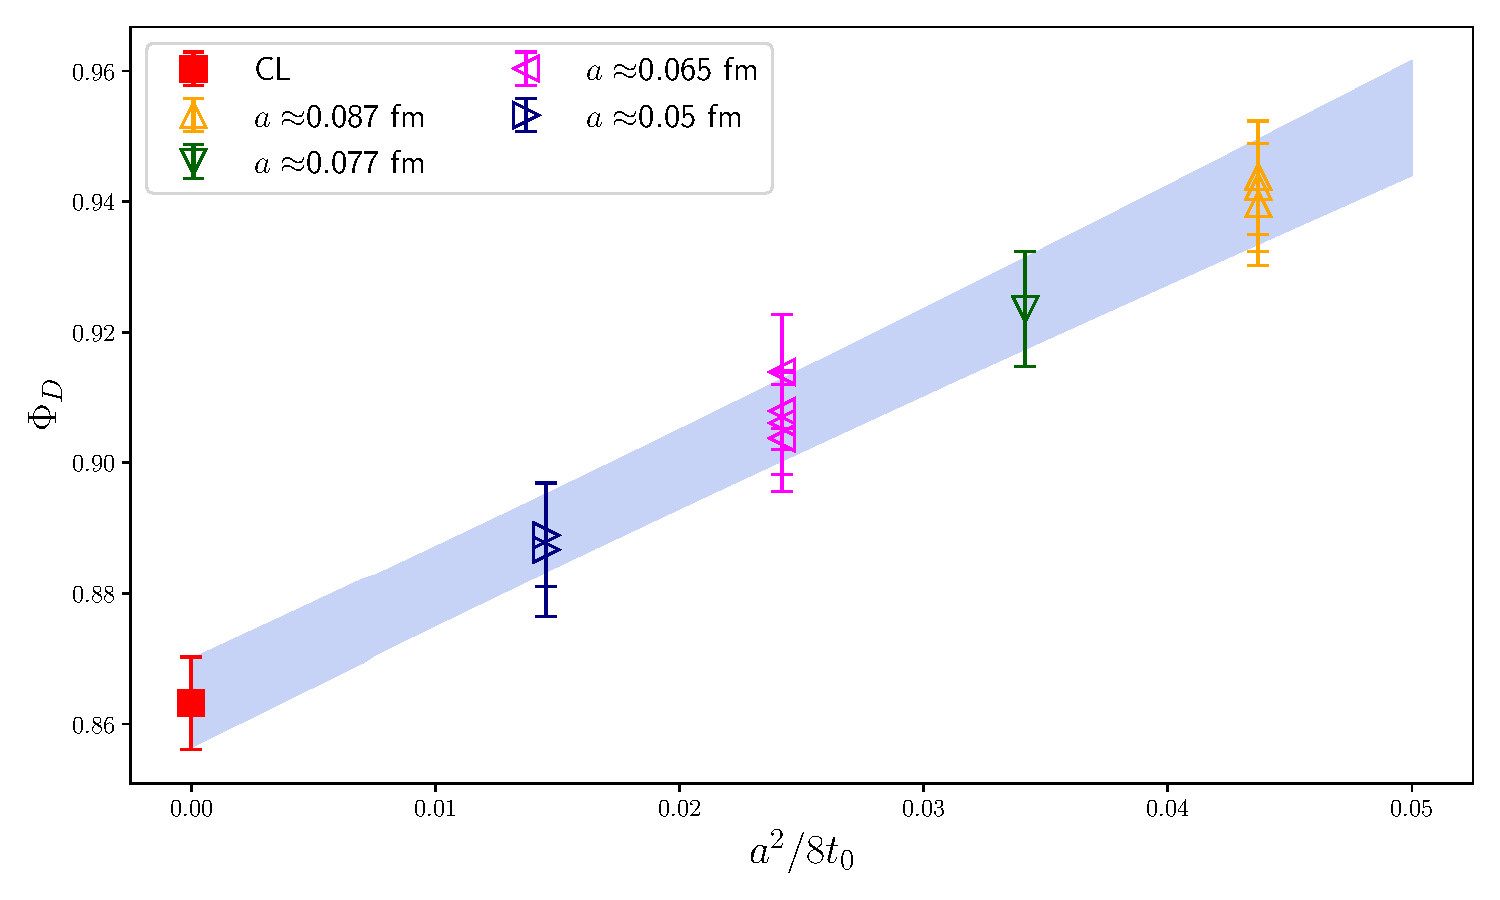
\includegraphics[scale=0.5]{./cap6/figs/fds/fit_cl_fD_fl_ave.pdf}
	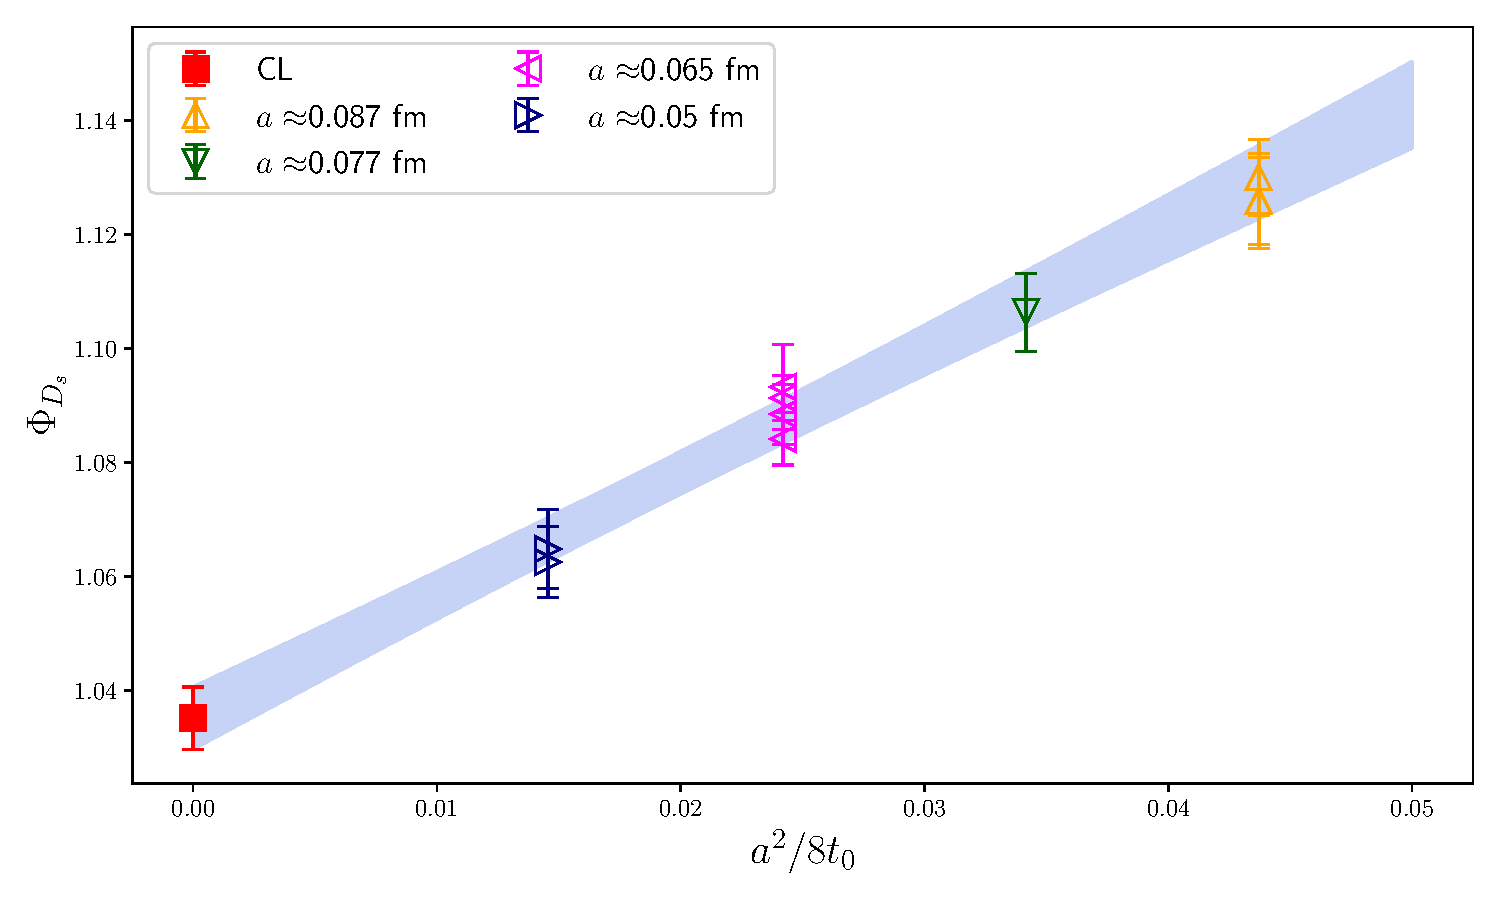
\includegraphics[scale=0.5]{./cap6/figs/fds/fit_cl_fDs_fl_ave.pdf}
	\caption{Continuum limit extrapolation of the best fits according to the TIC criteria applied to  $\Phi_D$ (\textit{top}) and $\Phi_{D_s}$ (\textit{bottom}).  Results are shown for the flavour-averaged matching condition $\phi_H^{(1)}$. The blue band represents the projection to the physical $\phi_2 = \phi_2^{\mathrm{phys}}$ and $\phi_H = \phi_H^{\mathrm{phys}}$, while the red square symbols denote the results in the continuum.}
	\label{fig:continuum_fits_fds}
\end{figure}

In Table~\ref{tab:dec_res_all_matching} we show our determinations of $\Phi_D$
and $\Phi_{D_s}$ for each of the two procedures to match the charm scale, as well
as the result from their combination. Using this combination we arrive at the following results for the the $D_{(s)}$ meson decay constants,
\begin{eqnarray}
	f_D &=& 211.3(1.9)(0.6) \ \mathrm{MeV},
	\\
	f_{D_s} &=& 247.0(1.9)(0.7) \ \mathrm{MeV},
\end{eqnarray}
where the first error is statistical and the second the systematic uncertainty from the model average.
The error budget for the $D_{(s)}$ decay constants is dominated by the statistical uncertainty of 
correlators and the  error on chiral-continuum extrapolations. Therefore, we expect that a future addition of other
ensembles with finer lattice spacing and physical pion masses will contribute to significantly reduce the uncertainty of our current 
determination. The different contributions to the variance of $D_{(s)}$ meson decay constants are 
shown in Figure~\ref{fig:fds_error_sources}. Finally, in  Figure~\ref{fig:fds_comparison} we show a comparison between our results and other $\NF=2+1$ lattice QCD determinations.
%
\begin{table}[t!]
	\begin{center}	
		\begin{tabular}{c ||  c c  c    }
			\hline
			&  $\phi_{H}^{(1)}$ & $\phi_{H}^{(2)} $  &  \text{combined} \\ [0.5ex]
			\hline\hline
			$\Phi_D$ &  0.8624(78)(7) & 0.8583(75)(8) &   0.8606(76)(21)   \\ [0.5ex]
			$\Phi_{D_s}$ & 1.0352(61)(9) & 1.0295(60)(11) &  1.0328(60)(30) 
		\end{tabular}
		\caption{Model average results for the observables $\Phi_D$ and $\Phi_{D_s}$ --- defined in Eq.~(\ref{eq:defphiD}) ---  which are related to the $f_D$ and $f_{D_s}$ decay constants, respectively, for
		the two different matching quantities $\phi_H^{(i)}$. The last column reports the result of the combination of these two matching conditions. The first error is statistical while the second is the estimate of systematic uncertainty arising from the model averaging procedure. }
		\label{tab:dec_res_all_matching}
	\end{center}
\end{table}

\begin{figure}[t!]
\begin{center}
\begin{minipage}{.40\linewidth}
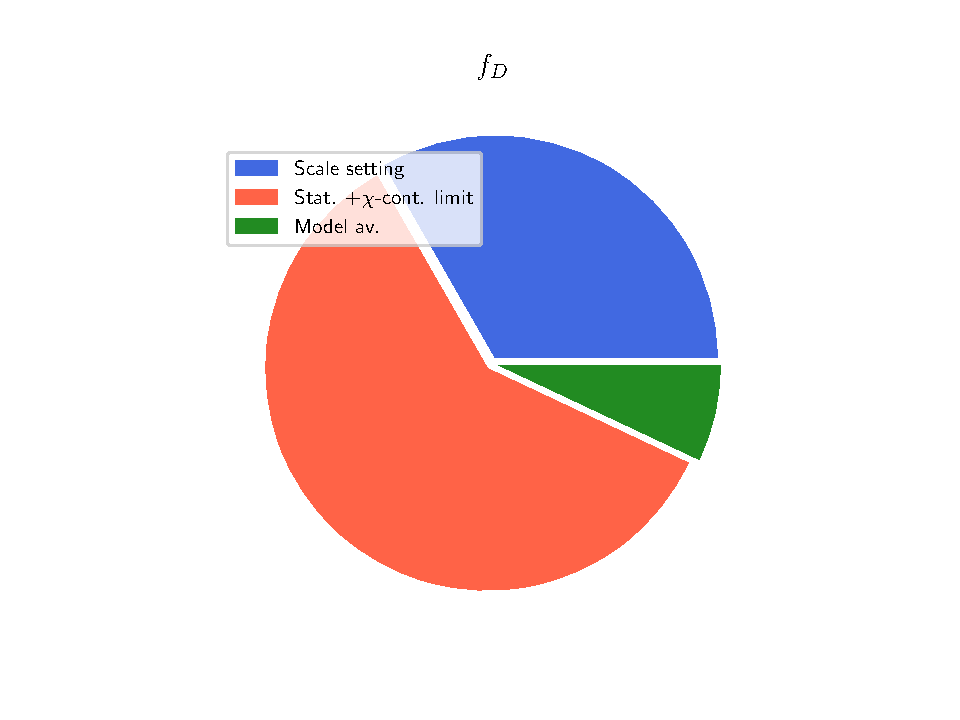
\includegraphics[width=\linewidth]{././cap6/figs/fds/error_pie_fd.pdf}
\end{minipage}
\hspace{10mm}
\begin{minipage}{.39\linewidth}
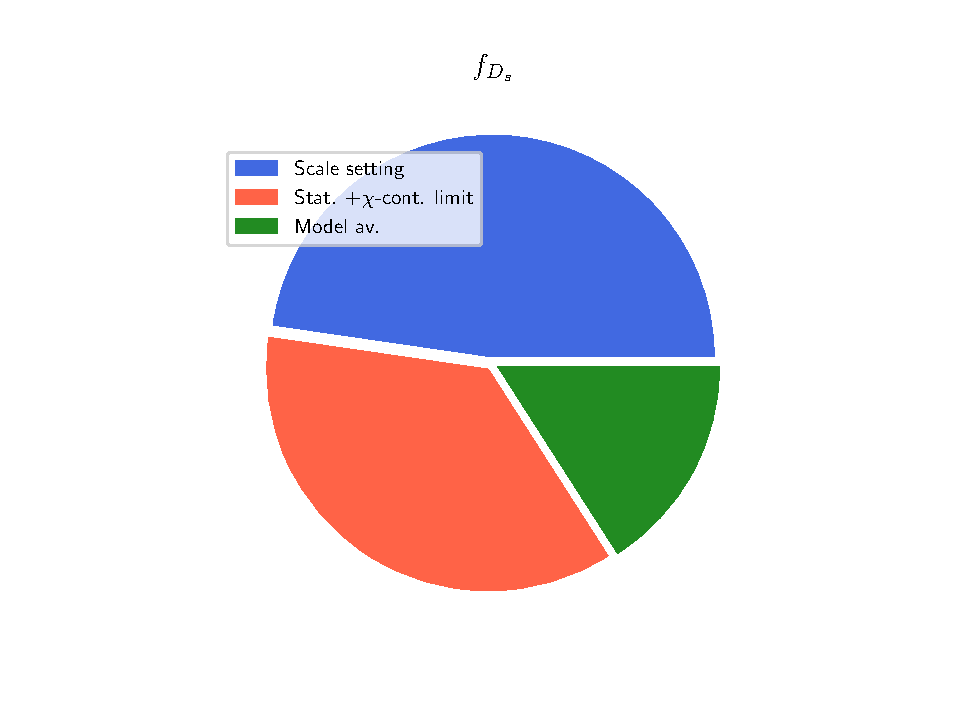
\includegraphics[width=\linewidth]{././cap6/figs/fds/error_pie_fds.pdf}
\end{minipage}
\end{center}
\vspace{-5mm}
	\caption{Relative contributions to the total error of our determinations of $f_D$ (\textit{left}) and $f_{D_s}$ (\textit{right}). The label statistical plus $\chi$-continuum limit represents the error arising from the statistical accuracy of our data and the chiral-continuum extrapolations. The scale setting label denotes the error coming from the physical value $t_0^{\mathrm{phys}}$ as determined within our setup \cite{MA1}, while the model average represents the systematic error arising from the model variation according to the TIC procedure.	}
	\label{fig:fds_error_sources}
\end{figure}


\begin{figure}[t!]
	\centering
	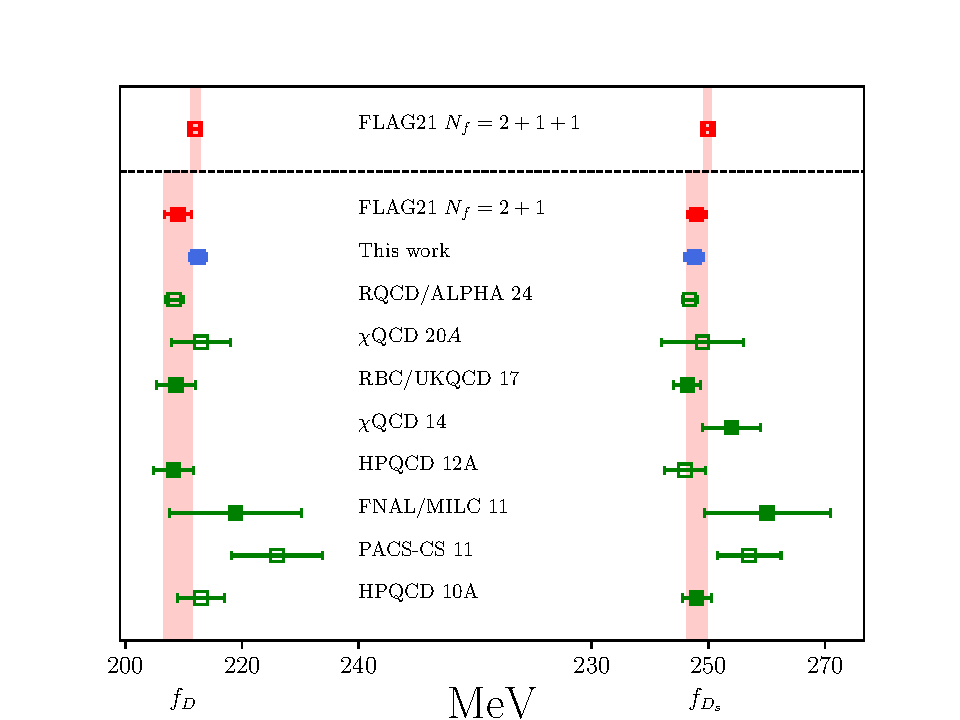
\includegraphics[scale=0.70]{./cap6/figs/fds/fds_comparison.pdf}
	\caption{Comparison of our results for $f_D$ and $f_{D_s}$  with those from lattice QCD collaborations based on simulations with $\NF=2+1$ dynamical flavours as well as with FLAG21 averages~\cite{FlavourLatticeAveragingGroupFLAG:2021npn}.
          Only data points with filled symbols contribute to  the FLAG averages. Starting from the bottom, results are taken from: HPQCD 10 \cite{Davies:2010ip}, PACS-CS 11 \cite{PACS-CS:2011ngu}, FNAL/MILC 11 \cite{FermilabLattice:2011njy}, HPQCD 12A \cite{Na:2012iu}, $\chi$QCD 14 \cite{Yang:2014sea}, RBC/UKQCD 17 \cite{Boyle:2017jwu},  $\chi$QCD 20A \cite{Chen:2020qma}.
          }
	\label{fig:fds_comparison}
\end{figure}

%%%

\subsection{Direct determination of $f_{D_s}/f_D$}

In addition to the determination of $f_D$ and $f_{D_s}$, we investigate the direct determination
of the ratio $f_{D_s}/f_D$ from a dedicated fit. This allows for a consistency check, since
the ratio is dimensionless and thus does not require normalisation with a reference scale
such as $\sqrt{8t_0}$. One particular consequence is thus that this approach is only
indirectly subject to the uncertainty of the lattice scale setting. Another advantage
is that the ratio is exactly~1 by construction when $m_s=m_l$, i.e., the symmetric
point of our $\phi_4={\rm constant}$ trajectory, which is part of our line of constant
physics. We can thus perform a fit that is highly constrained in the unphysical masses
region, although at the price of reducing the total number of ensembles entering in the study of the approach to the physical point.

A first set of fit ansaetze is derived from the HM$\chi$PT expressions considered above
for $\Phi_{D_{(s)}}$. The generic form is
\begin{equation}
	\frac{\Phi_{D_s}}{\Phi_D} = \left[
	1 + \left(
	\delta\Phi_{\chi\mathrm{PT}}^{D_s} - \delta\Phi_{\chi\mathrm{PT}}^{D}
	\right)
	\right]
	\left[
	1 + \left(
	\delta\Phi_{a}^{D_s} - \delta\Phi_{a}^{D_s}
	\right)
	\right].
	\label{eq:ratio_fds_expansion}
\end{equation}
Here $\delta\Phi_{\chi\mathrm{PT}}^{D_{(s)}}$  introduced in Eq.~(\ref{eq:deltaphichis}) labels the light quark mass dependence of the ratio, while $\delta\Phi_a^{D_{(s)}}$ from Eq.~(\ref{eq:phias}) controls the continuum approach. It is worth noticing that at leading order the physical dependence on $\phi_H$, and also the lattice spacing dependence related to $\phi_H$, cancel out when expanding the ratio.
Collecting all the terms entering in Eq.~(\ref{eq:ratio_fds_expansion}) from the previous section,
we end up with 
\begin{equation}
	\begin{split}
		\frac{\Phi_{D_s}}{\Phi_D} =&
		\left[  1 - \frac{1+3g^2}{64\pi^2 \phi_f^2} \left[ 2 \mathcal{L}_{K} + \mathcal{L}_{\eta} - 3 \mathcal{L}_{\pi} \right] 
		+ \frac{4 \left( 2\phi_4 - 3 \phi_2 \right)}{\phi_f^2}  \left( p_\chi^{(0)} +  p_\chi^{(2)} \frac{\phi_2}{\phi_f^2} + \frac{p_\chi^{(4)}}{\phi_H} \right)  \right]  
		\\
		&\times \left[ 1+ \frac{a^2}{8t_0} \left( 2 \phi_4 - 3 \phi_2 \right) \left( p_a^{(1)} + p_a^{(3)} \phi_H^2 \right)  \right]. 
		\label{eq:ratiophi}
	\end{split}
\end{equation}
In this expression we consider all the possible combinations of non-vanishing fit parameters,
and perform our TIC-weighted model average among the different functional forms tested to
quote a systematic uncertainty.  

Given that various terms cancel in the  HM$\chi$PT expressions, we will further explore the systematic uncertainties by considering  also functional forms based on a Taylor expansion of $\Phi_{D_{(s)}}$. The generic
expression then reads
\begin{align}
	\Phi_{D_{(s)}}= \left( \Phi_{D_{(s)}}\right)_{\chi} \left[ 1 + \delta \Phi_{{h,\mathrm{Taylor}}} \right] \left[ 1 + \delta \Phi_{{m,\mathrm{Taylor}}}^{D_{(s)}} \right] \left[ 1 + \delta \Phi_a^{D_{(s)}}  \right]
	\,,
	\label{eq:phiqcontT}
\end{align}
where $ \left( \Phi_{D_{(s)}}\right)_{\chi}$ is the value in
the chiral limit and at the physical value of the heavy-quark mass.
In this expansion, the heavy and light mass dependence terms read
\begin{equation}
	\begin{split}
		\delta \Phi_{{h,\mathrm{Taylor}}} &=  p_h^{(0)} \left( \frac{1}{\phi_H} - \frac{1}{\phi_H^{\mathrm{phys}}} \right) + p_h^{(1)} \left( \frac{1}{\phi_H} - \frac{1}{\phi_H^{\mathrm{phys}}} \right)^2 ,
		\\
		\delta \Phi_{{m,\mathrm{Taylor}}}^{D} &=  p_m^{(0)} \phi_4 + \phi_2 \left[ p_m^{(1)}  +  p_m^{(2)} \phi_2 + p_m^{(3)} \left( \frac{1}{\phi_H} - \frac{1}{\phi_H^{\mathrm{phys}}} \right)  \right] ,
		\\
		\delta \Phi_{{m,\mathrm{Taylor}}}^{D_s} &=  p_m^{(0)} \phi_4 + 2 (\phi_4 - \phi_2)  \left[ p_m^{(1)}  + p_m^{(2)} \phi_2 + p_m^{(3)} \left( \frac{1}{\phi_H} - \frac{1}{\phi_H^{\mathrm{phys}}} \right)  \right].
		\label{eq:deltaphiTs} 
	\end{split}
\end{equation}
The lattice spacing dependence  $\delta \Phi_{a}^{D_{(s)}}$ can be parameterised in a similar fashion to that in \req{eq:phias}.
Combining these expressions into a functional form for the ratio of decay constants one then has
\begin{align}
	\frac{\Phi_{D_s}}{\Phi_D}   =& \left[  1 +  \left( 2 \phi_4 - 3 \phi_2 \right)  \left[ p_m^{(1)}  +  p_m^{(2)} \phi_2 + p_m^{(3)} \left( \frac{1}{\phi_H} - \frac{1}{\phi_H^{\mathrm{phys}}} \right) \right]  \right]  
	\nonumber \\
	& \times \left[ 1+ \frac{a^2}{8t_0}  \left( 2 \phi_4 - 3 \phi_2 \right) \left( p_a^{(1)} + p_a^{(3)} \phi_H^2 \right)  \right] \,.
	\label{eq:ratiophiT}
\end{align}

Then, in order to arrive at a final determination of $f_{D_s}/f_D$ we perform a model average among all the HM$\chi$PT and Taylor functional forms for the two different matching conditions simultaneously. In Table~\ref{tab:ratio_res_all_matching} we report our results for the
ratio of decay constants from the model average separately for each charm matching
condition, as well as their combination. Also for the ratio we observe good agreement for the two different $\phi_H^{(i)}$ tested in this work. 
Finally, for the  result combining the two matching conditions, we quote 
\begin{equation}
	\frac{f_{D_s}}{f_D} = 1.177(15)(5),
\end{equation}
where  the first error is  statistical and the second is the systematic uncertainty based on  the model average procedure. 

In Figure~\ref{fig:fds_ratio} we show the HM$\chi$PT chiral-continuum fit of the 
$\Phi_{D_s}/\Phi_D$ ratio with highest weight in the model averaging procedure. In particular the plot on the left shows the chiral approach to the physical point, 
while the plot on the right represents the lattice spacing dependence.
The observed dependence on $\phi_2$ shows only a mild curvature arising from the chiral logs, while cutoff effects appear to be highly suppressed at the current level of statistical precision of our data.

\begin{figure}[!htb]
	\centering
	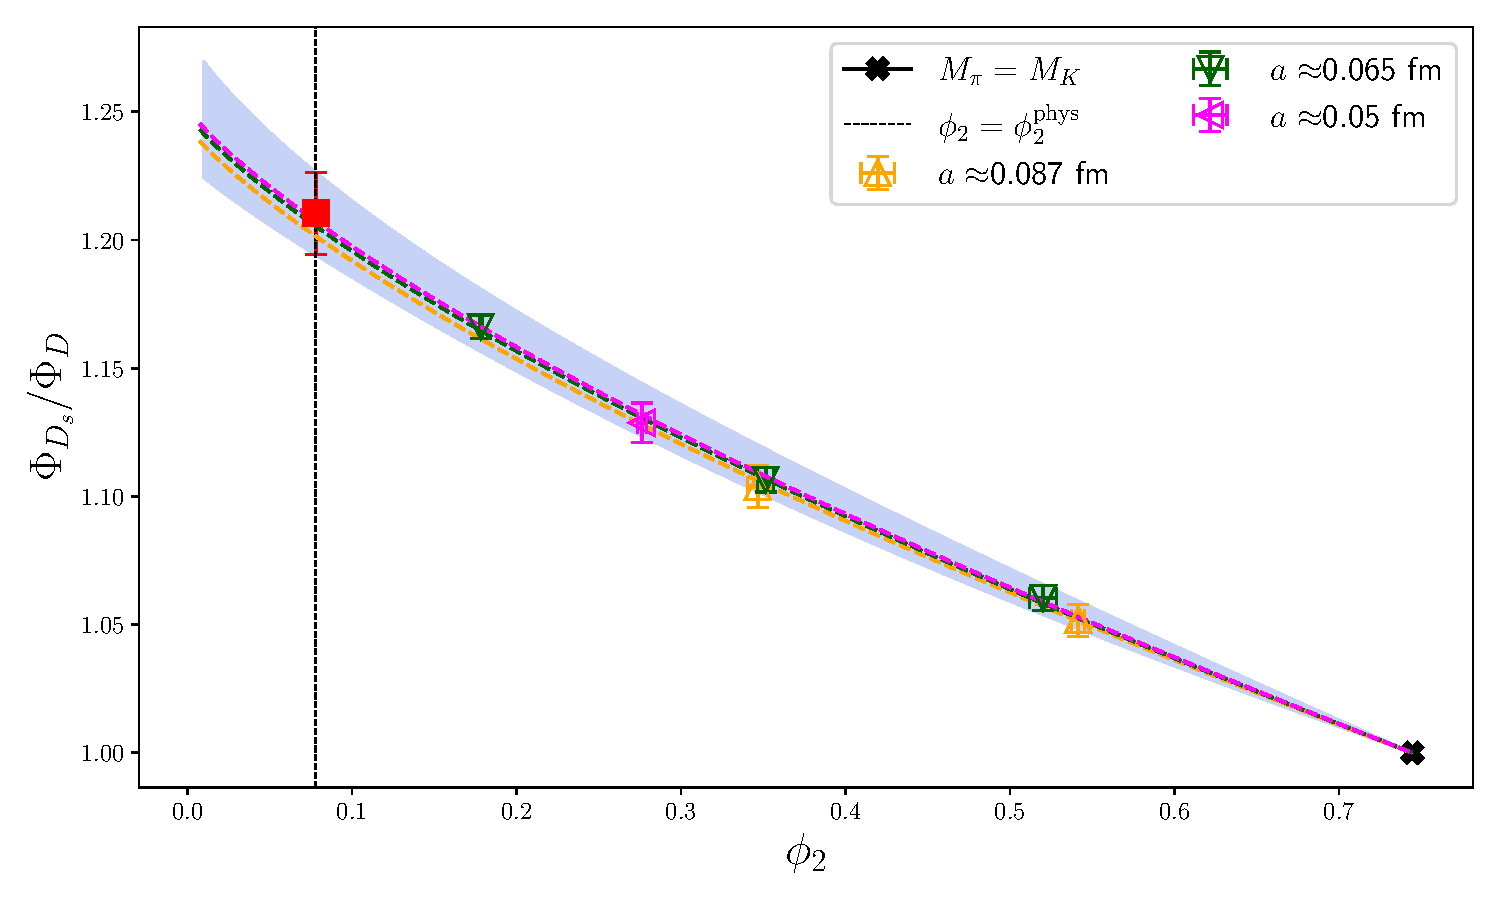
\includegraphics[scale=0.50]{./cap6/figs/fds/fit_fds_ratio_fds_over_fd.pdf}
	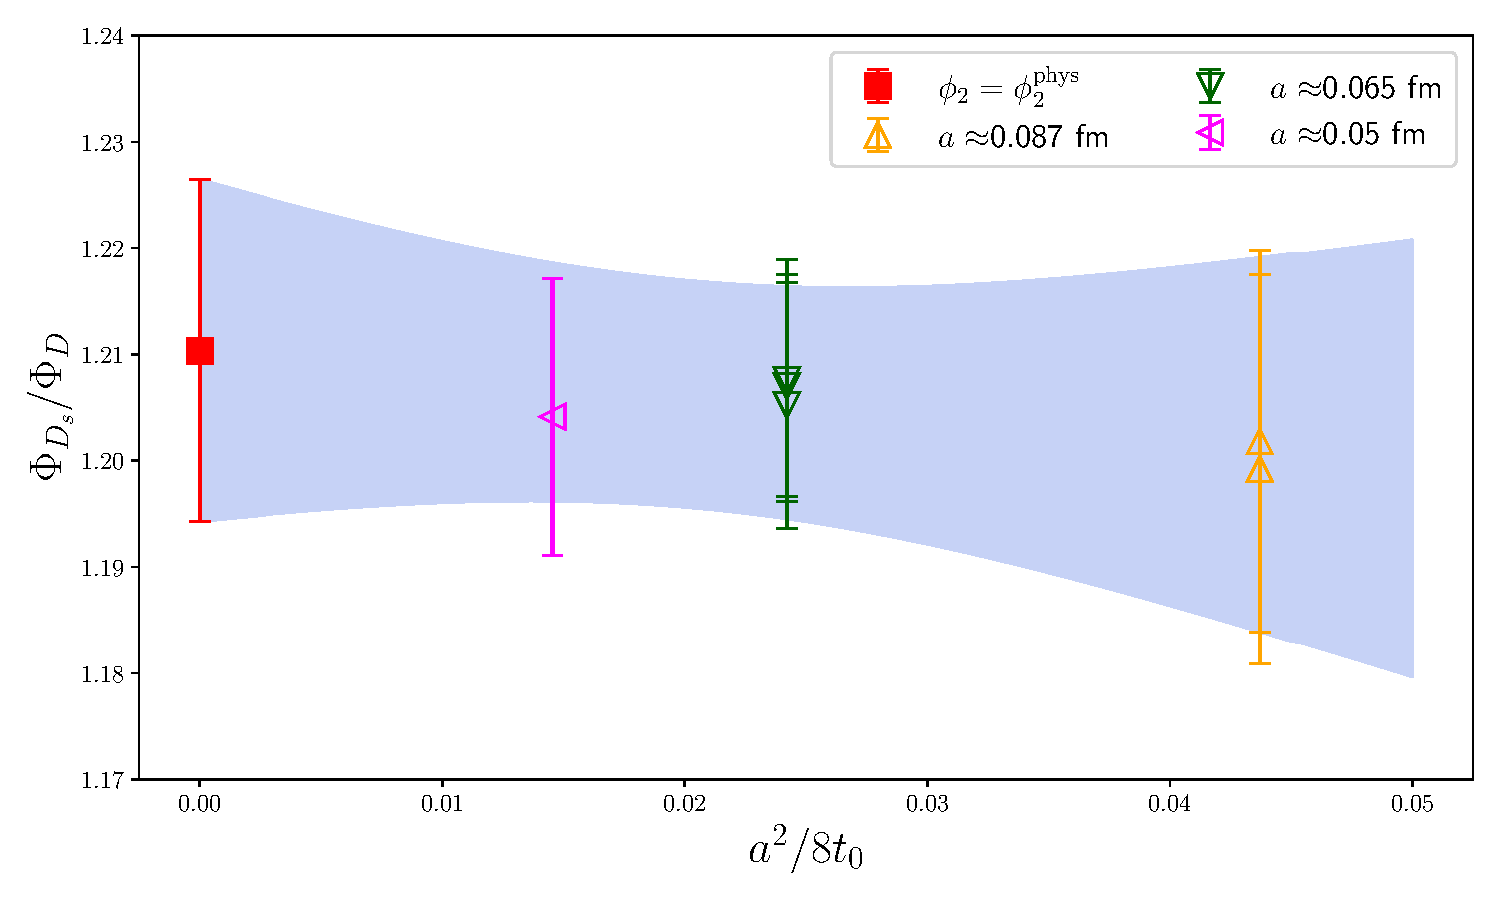
\includegraphics[scale=0.50]{./cap6/figs/fds/fit_cl_fds_ratio_fds.pdf}
	\caption{Illustration of the chiral-continuum extrapolation of the ratio $\Phi_{D_s}/\Phi_D$ for the HM$\chi$PT model with highest TIC value. Results are shown for the flavour-averaged matching condition. \textit{Top}:  Chiral approach to the physical point. The dashed lines illustrate the chiral trajectories at finite lattice spacing, while the blue shaded band is a projection of the continuum fit. The red square symbol represents the physical result in the continuum. The black cross symbol corresponds to the symmetric point. Data points at finite lattice spacing are projected to the physical charm quark mass. \textit{Bottom}: Lattice spacing dependence of  $\Phi_{D_s}/\Phi_D$. The red square symbol indicates the continuum result, while the blue shaded band shows the fitted functional dependence on the lattice spacing.  Points at finite lattice spacing are projected to the physical values of $\phi_2$ and $\phi_H$.}
	\label{fig:fds_ratio}
\end{figure}

 Figure~\ref{fig:fds_ratio_model_av}
shows a summary of the model average procedure for the ratio $\Phi_{D_s}/\Phi_D$, displaying the fit results for the two 
matching conditions together with the associated weights, for the HM$\chi$PT and Taylor functional forms.

\begin{table}[t!]
	\begin{center}	
		\begin{tabular}{c ||  c c  c}
			\hline
			 &  $\phi_{H}^{(1)}$ & $\phi_{H}^{(2)} $   & combined \\ [0.5ex]
			\hline\hline
			$f_{D_s}/f_D$   &  1.177(15)(6)& 1.178(15)(6) &  1.177(15)(5)
		\end{tabular}
		\caption{Results of the model average for $f_{D_s}/f_D$ for the two charm-quark matching conditions. The last column reports the combined result. The first error is statistical while the second is the systematic uncertainty arising from the model variation procedure. }
		\label{tab:ratio_res_all_matching}
	\end{center}
\end{table}
  In Figure \ref{fig:fds_ratio_error}  we show the major error sources contributing to our final determination of the ratio, where we notice that the major contribution is given by the statistical and chiral-continuum error. Finally, in Figure \ref{fig:fds_over_fd_comparison} we show a comparison between our result for $f_{D_s}/f_D$, the FLAG21 average and results from other collaborations.


\begin{figure}[!t]
	\centering
	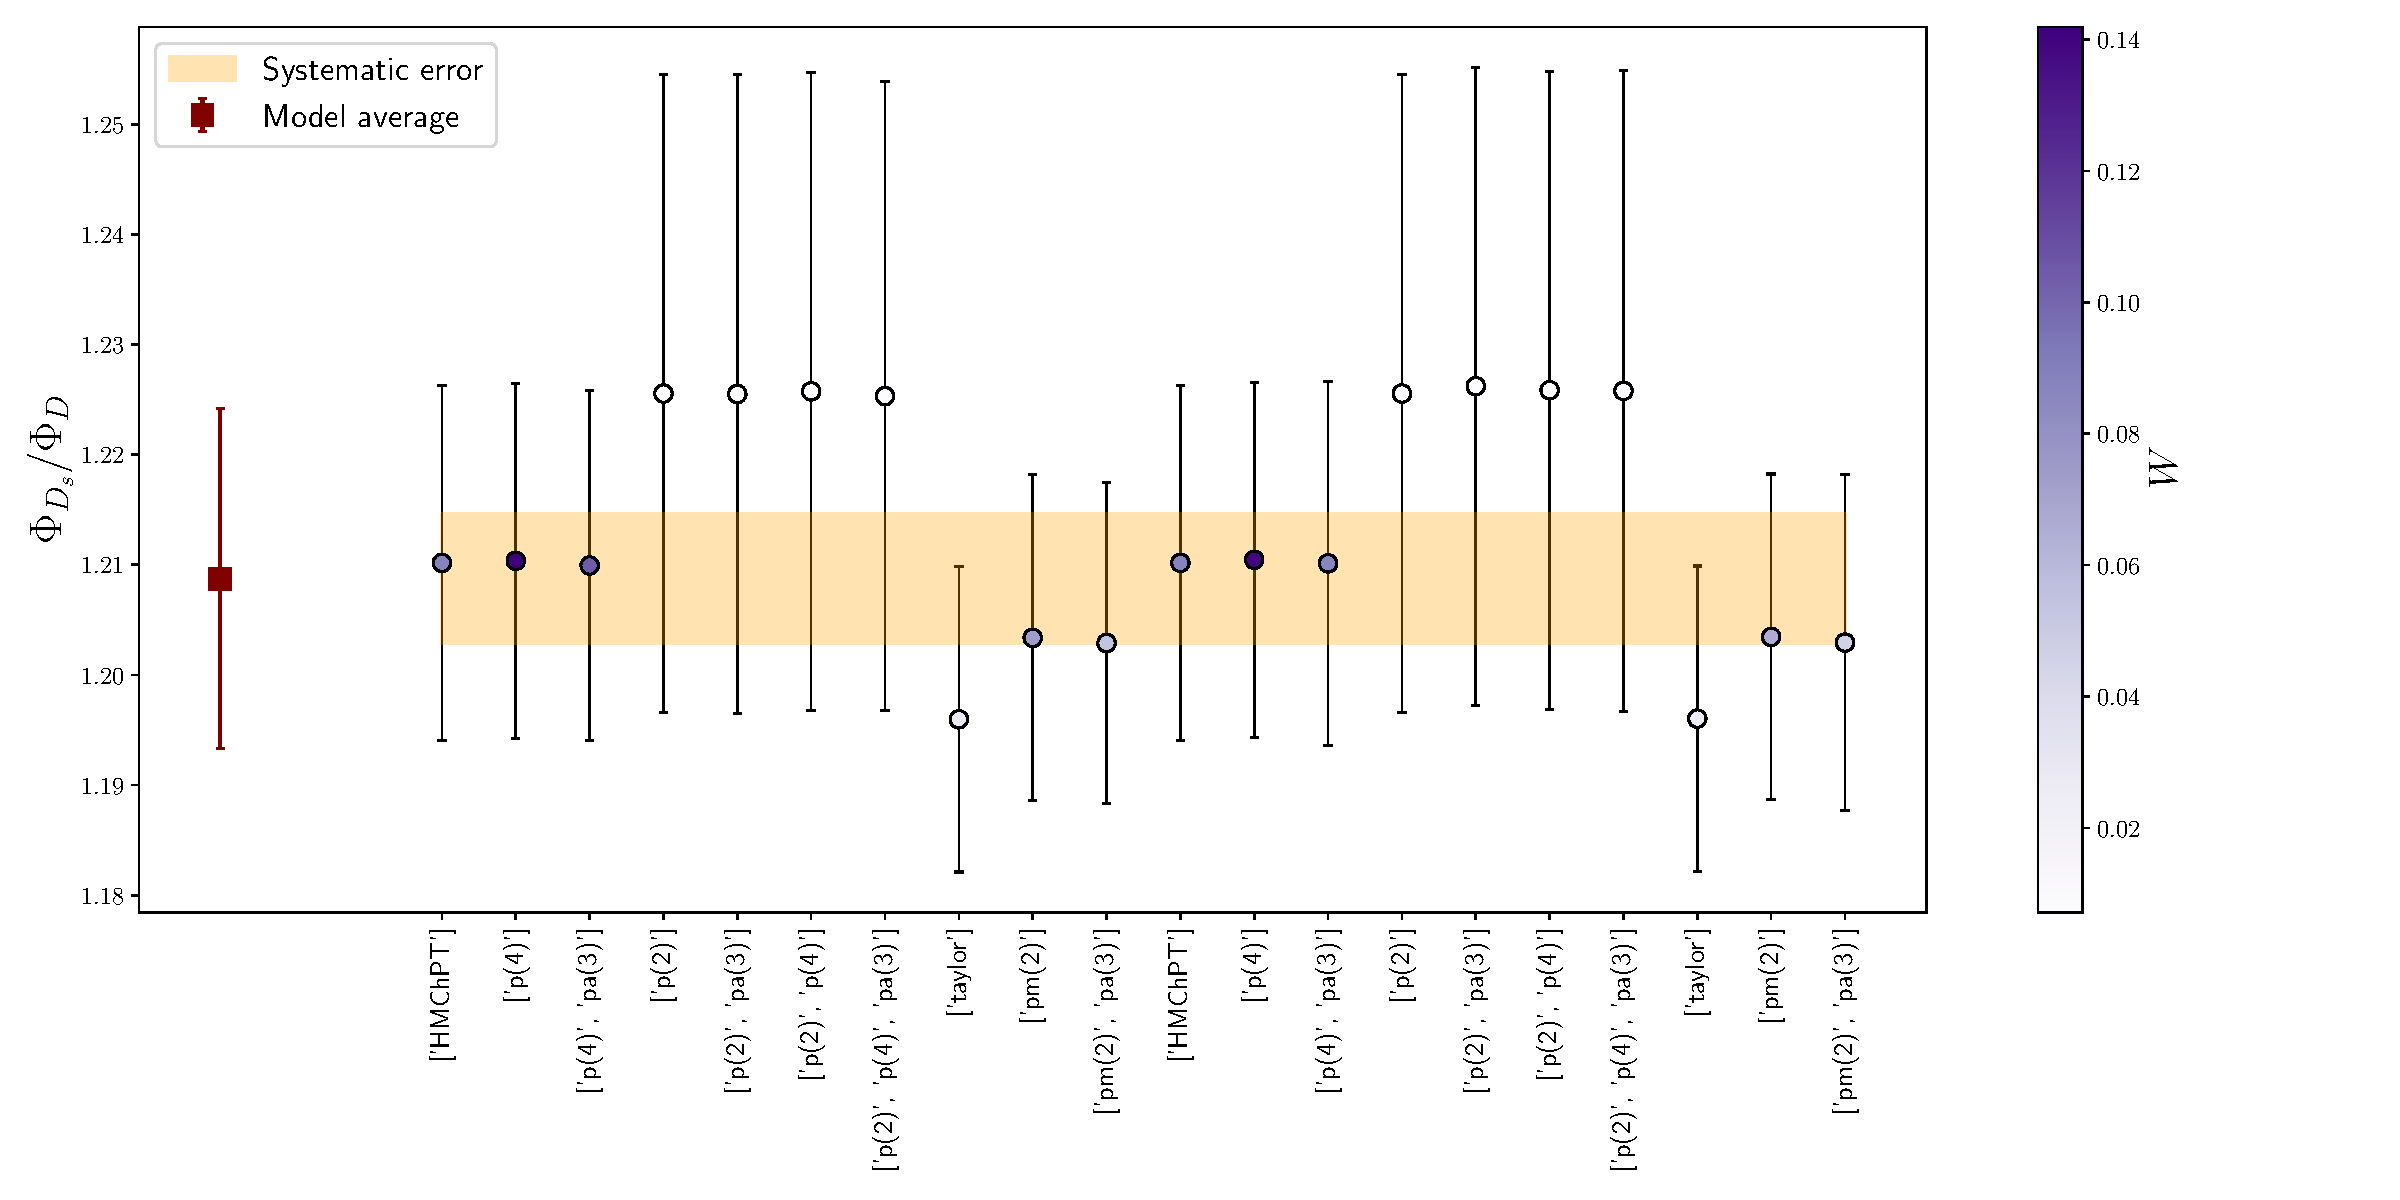
\includegraphics[scale=0.4]{./cap6/figs/fds/cat_ave_totfds_over_fd.pdf}
	\caption{Summary of the model average procedure for the ratio $\Phi_{D_s}/\Phi_D$ based on the combination of the two matching conditions, $\phi_{H}^{(1)}$ and $\phi_{H}^{(2)}$. Each circular symbol  represents the result of a specific functional form, and the opacity is associated to the normalised weight $W$ of the model based on its TIC value. The yellow band represents the systematic uncertainty arising from the set of tested models, while the left-most red point is our final  averaged result. The labels of the 20 models specified in the horizontal axis are related to the terms characterising the dependencies on the mass and lattice spacing in the following way:  \texttt{`HMChPT'}  stands for the expression in Eq.~(\ref{eq:ratiophi}) where only the leading terms depending on the fit parameters $p_\chi^{(0)}$ and $p_a^{(1)}$ are considered . Similarly,  \texttt{`taylor'} refers to Eq.~(\ref{eq:ratiophi}) where only the terms depending on the fit parameters $p_m^{(1)}$ and $p_a^{(1)}$ are kept. The labels \texttt{`p(2)'} and \texttt{`p(4)'} correspond to the addition of the higher order terms depending on the parameters $p_\chi^{(2)}$ and   $p_\chi^{(4)}$ in Eq.~(\ref{eq:ratiophi}), respectively, while  \texttt{`pm(2)'} denotes the addition of $p_m^{(2)}$ from Eq.~(\ref{eq:ratiophiT}). Finally,  \texttt{`p(3)'}  denotes the inclusion of the fit parameter $p_a^{(3)}$ parameterising  higher order  lattice spacing dependence appearing in both the HM$\chi$PT and Taylor functional forms in Eq.~(\ref{eq:ratiophi}) and Eq.~(\ref{eq:ratiophiT}).
        } 
	\label{fig:fds_ratio_model_av}
\end{figure}

\begin{figure}[!h]
\begin{center}
\begin{minipage}{.43\linewidth}
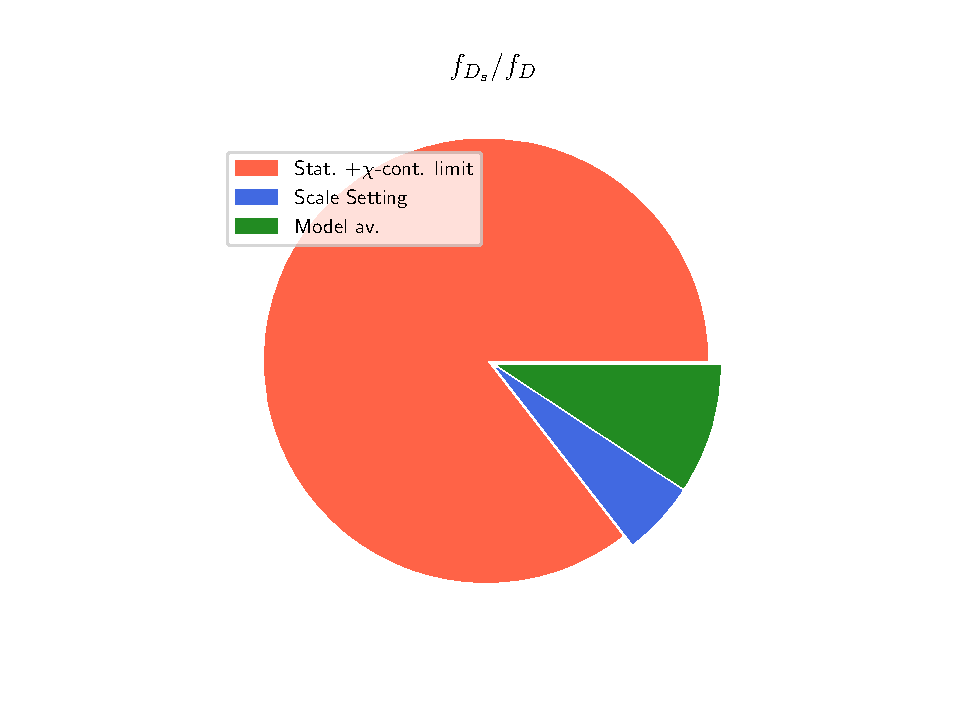
\includegraphics[width=\linewidth]{././cap6/figs/fds/error_pie_ratio_fds.pdf}
\end{minipage}
\hspace{15mm}
\begin{minipage}{.4\linewidth}
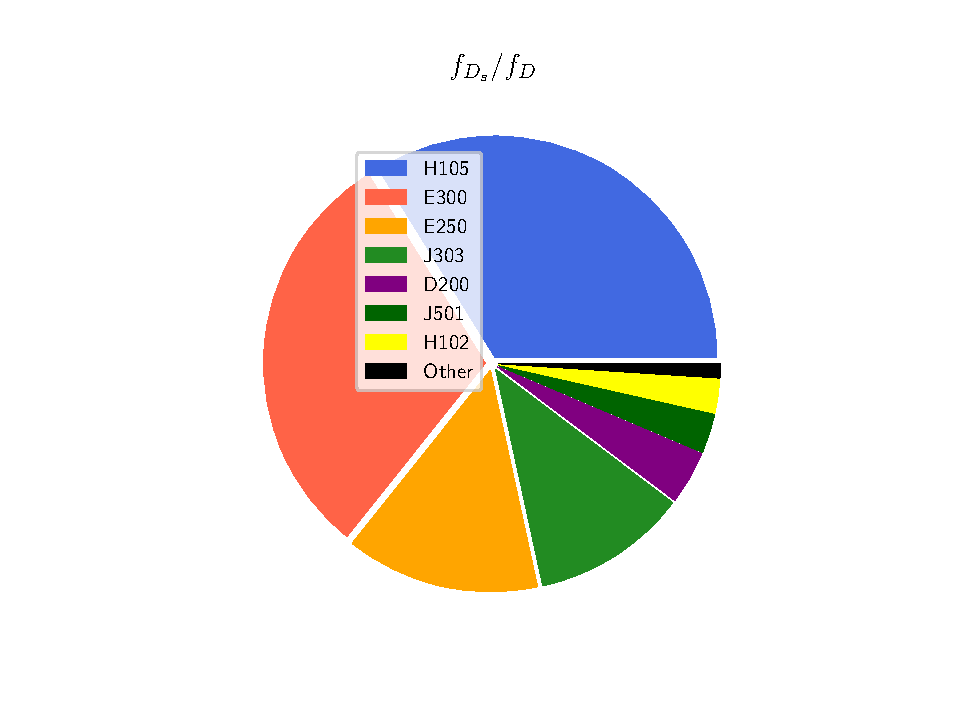
\includegraphics[width=\linewidth]{././cap6/figs/fds/error_pie_ratio_fds_statonly.pdf}
\end{minipage}
\end{center}
\vspace{-5mm}
	\caption{\textit{Left}: Relative contributions to the total error on the determination of the ratio $f_{D_s}/f_D$. The label statistical plus $\chi$-continuum limit represents the error arising from the statistical accuracy of our data and the chiral-continuum extrapolation. The scale setting label denotes the error coming from the physical value $t_0^{\mathrm{phys}}$, while the model average represents the systematic error arising from the model variation according to the TIC procedure. \textit{Right}: Details of the relative contributions to the statistical and chiral-continuum extrapolation error arising from specific gauge field configuration ensembles. 
          }
	    \label{fig:fds_ratio_error}
\end{figure}

\begin{figure}[!h]
	\centering
	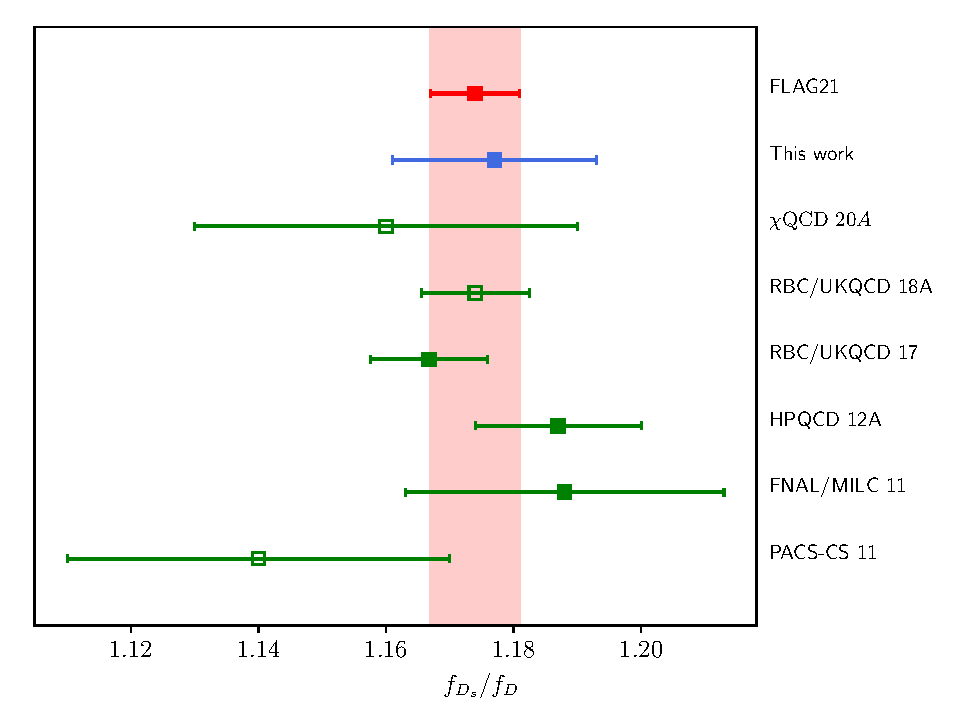
\includegraphics[scale=0.7]{./cap6/figs/fds/ratio_fds_comparison.pdf}
	\caption{Comparison of our determination of $f_{D_s}/f_D$ with those of the other lattice QCD collaborations based on $\NF=2+1$ dynamical simulations as well as with the FLAG average~\cite{FlavourLatticeAveragingGroupFLAG:2021npn}. Only the results with filled symbols contribute to this average. Starting from the bottom, results are taken from:  PACS-CS 11 \cite{PACS-CS:2011ngu}, FNAL/MILC 11  \cite{FermilabLattice:2011njy}, HPQCD 12A \cite{Na:2012iu},  RBC/UKQCD 17 \cite{Boyle:2017jwu}, RBC/UKQCD 18A \cite{Boyle:2018knm},  $\chi$QCD 20A \cite{Chen:2020qma}. }
	\label{fig:fds_over_fd_comparison}
\end{figure}





%%%%%%%%%%%%%%%%%%%%%%%%%%%%%%%%%%%%%%%%%%%%%%%%%%%%%%%%%%%
%%%%%%%%%%%%%%%%%%%%%%%%%%%%%%%%%%%%%%%%%%%%%%%%%%%%%%%%%%%
